\documentclass[12pt]{book}

\usepackage[a4paper,outer=1.4in,inner=0.8in,vmargin=3cm]{geometry}

\usepackage[utf8]{inputenc}

\usepackage{wrapfig}
\usepackage{pdflscape}
\usepackage{natbib}
\usepackage{graphicx}
\usepackage{amsthm}
\usepackage{amsmath}
\usepackage{setspace}
\usepackage{color}
\usepackage{lmodern}
\usepackage{float}
\restylefloat{table}

\usepackage{sidecap}
\usepackage[scaled]{helvet}
\usepackage{caption}


\setlength{\marginparwidth}{1in}

\newcounter{todos}
\newcounter{comments}
\newcounter{figcomments}
\newcounter{advisorcomments}
\newcounter{questions}

\setcounter{tocdepth}{4}

\definecolor{grey}{rgb}{0.4,0.4,0.4}
\definecolor{brown}{rgb}{0.5,0.0,0.0}
\definecolor{orange}{rgb}{0.7,0.3,0.}
\DeclareCaptionFont{grey}{\color{grey}}
\captionsetup{margin=10pt,font=small,labelfont=bf,format=plain,textfont=grey,labelfont=grey}

\renewcommand*\familydefault{\sfdefault} %% Only if the base font of the document is to be sans serif
\usepackage[T1]{fontenc}
\linespread{1.2}

\title{Demonstrating Quantum Speed-Up with a Two-Transmon Quantum Processor.}
\author{Andreas Dewes}

\theoremstyle{definition}
\newtheorem{theorem}{Theorem}[chapter]
\newtheorem{axiom}{Axiom}[theorem]

\newcommand{\bracket}[1]{\left< #1 \right>} % for Dirac brackets
\newcommand{\ket}[1]{\left| #1 \right>} % for Dirac bras
\newcommand{\bra}[1]{\left< #1 \right|} % for Dirac kets
\newcommand{\todo}[1]{
  \addtocounter{todos}{1}
	\textcolor{red}{!\arabic{todos}!}
	\marginpar{
		\begin{spacing}{0.5}
			\textcolor{red}
				{
				{\flushleft \scriptsize  \linespread{0.8} To Do \arabic{todos}: #1}
				}
		\end{spacing}
	}
}
\newcommand{\figcomment}[1]{
	%To do: Fix the bug that makes the counter value increase by 2 each time this command is called.
	\addtocounter{figcomments}{1}
	\textcolor{orange}{Figure Comment \arabic{figcomments}: #1}
}

\newcommand{\comment}[1]{
  \addtocounter{comments}{1}
	\textcolor{orange}{!\arabic{comments}!}
	\marginpar{
		\begin{spacing}{0.5}
			\textcolor{orange}
				{
				{\flushleft \scriptsize  \linespread{0.8} Comment \arabic{comments}: #1}
				}
		\end{spacing}
	}
}

\newcommand{\question}[1]{
  \addtocounter{questions}{1}
	\textcolor{blue}{?\arabic{questions}?}
	\marginpar{
		\begin{spacing}{0.5}
			\textcolor{blue}
				{
				{\flushleft \scriptsize  \linespread{0.8} Question \arabic{questions}: #1}
				}
		\end{spacing}
	}
}

\newcommand{\advisorcomment}[1]{
  \addtocounter{advisorcomments}{1}
	\textcolor{yellow}{!\arabic{advisorcomments}!}
	\marginpar{
		\begin{spacing}{0.5}
			\textcolor{yellow}
				{
				{\flushleft \scriptsize  \linespread{0.8} Advisor comment \arabic{advisorcomments}: #1}
				}
		\end{spacing}
	}
}

\begin{document}

\maketitle

\tableofcontents

\listoffigures

\listoftables

\chapter{Introduction \& Summary}

%Provide a short summary of the whole PhD thesis:
% -Introduction to QC & CQED
% -Building Blocks of Superconducting Quantum Processors
% -Realization of a Two-Transmon QP
% -Tune-Up & Characterization of the Universal Two-Qubit Gate
% -Grover's Algorithm: Introduction & Background
% -Implementation on the Two-Qubit Processor
% -Design of a Scalable QC Architecture

\section{Quantum Computing \& Circuit Quantum Electrodynamics}

\begin{figure}
	\centering
		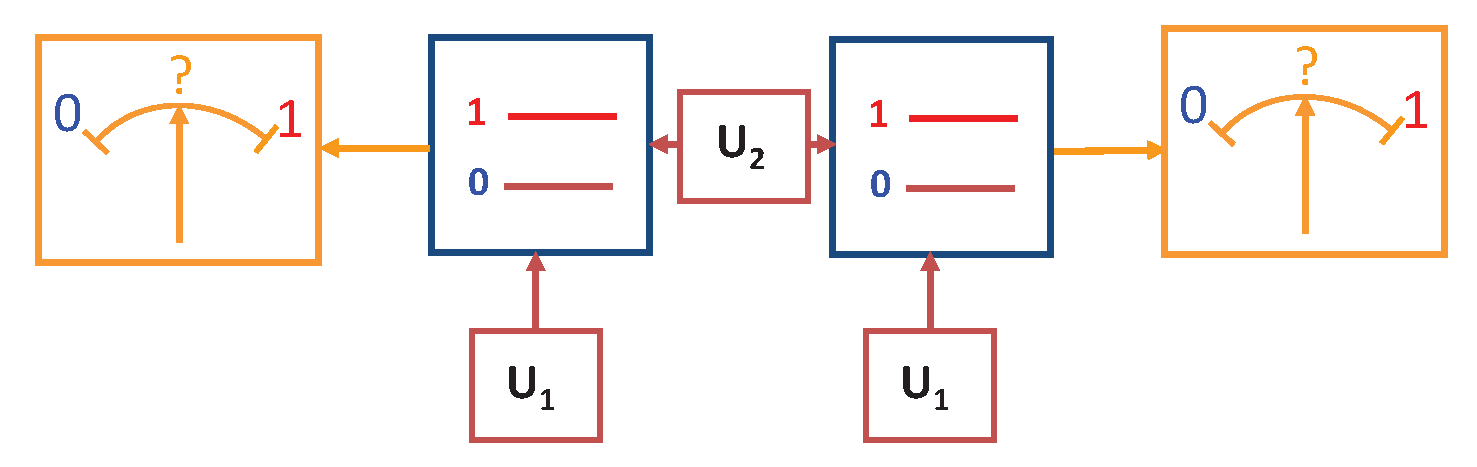
\includegraphics[width=0.8\textwidth]{./material/papers/grover/submission1/Fig1}
	\caption[Blueprint of a two-qubit quantum processor]{The blueprint of a two-qubit quantum processor. Shown are two qubits that can be individually manipulated ($U_1$) and are connected by a universal two-qubit gate $U_2$. Each of the qubits can be read out individually.}
	\label{fig:qubit_processor_blueprint}
\end{figure}

This thesis presents experiments performed with a superconducting two-qubit quantum processor. The main goal of this work was to demonstrate a possible quantum computing architecture using superconducting qubits that follows the canonical blueprint of a quantum processor as shown in fig. \ref{fig:qubit_processor_blueprint}, following the four criteria formulated by \cite{divincenzo_physical_2000}. Following this definition, a universal quantum computer is a register of quantum bits -- or qubits -- on which one can perform universal single- and two-qubit quantum gates, read out the state of each qubit individually and with high fidelity and reset the qubit register to a well-defined state.

Implementing this allegedly simple list of requirements in a system of superconducting qubits has been a major research challenge during the last decade. The first demonstration of coherent quantum dynamics in a superconducting charge-based qubit by \cite{nakamura_coherent_1999} opened up a broad research field on superconducting quantum bits. In the years following Nakamuras initial experiment, several types of superconducting qubits were proposed and realized using e.g. the superconducting phase \citep{martinis_energy-level_1985,martinis_rabi_2002} across a Josephson junction or the magnetic flux \citep{mooij_josephson_1999,chiorescu_coherent_2003} inside a superconducting ring interrupted by one or several Josephson junctions as the dominant quantum variable. An important result on the way to the development of robust superconducting qubits was the development of the so-called {\it Quantronium} qubit by \cite{vion_manipulating_2002}, which achieved quantum-mechanical coherence times larger than 1 $\mu s$, made possible by operating a Cooper pair box at a sweet spot in a regime where the charging and Josephson phase energies of the system are of comparable value. The high coherence times achieved with this qubit made it possible to perform --for the first time-- robust, NMR-like quantum operations using a superconducting qubit \citep{collin_nmr-like_2004}. Then, in 2004, the development of a new type of qubit, the so called {\it Transmon} by \cite{wallraff_strong_2004} marked again a drastic improvement in coherence times. By decreasing the charging energy of a Cooper pair box and thus operating the device in the phase regime, the resulting qubit becomes quasi insensitive to charge noise. Furthermore, by embedding the Transmon qubit in a superconducting coplanar waveguide (CPW) resonator it is possible to protect it from external sources of electrical noise and to use the dirspersive interaction between the qubit and the resonator for reading out the qubit state\citep{blais_cavity_2004}. With this so-called {\it circuit quantum electrodyanmics} (CQED) architecture, quantum gates and algorithms with up to three qubits have been implemented so-far, demonstrating multi-qubit entanglement \citep{dicarlo_preparation_2010} and simple quantum algorithms \citep{dicarlo_demonstration_2009}.

\todo{Think about moving the section on 3D-CQED directly after this one since this would probably be more logical}

In parallel to this, the development of reliable quantum-limited amplifiers based on nonlinear superconducting resonators by \question{Should I mention Michel here?}I. Siddiqi \citep{siddiqi_rf-driven_2004,vijay_invited_2009} complemented the CQED architecture by providing a fast and high-fidelity readout scheme for Transmon qubits \citep{siddiqi_dispersive_2006,mallet_single-shot_2009} and for the amplification of quantum signals in general\todo{Add more citations here}. These quantum-limited amplifiers and detectors made it possible to directly observe quantum jumps in superconducting qubits \citep{vijay_observation_2011} and to implement simple quantum feedback schemes in superconducting circuits\todo{Add reference to quantum feedback paper as soon as it appears}.

Recently, the development of a CQED architecture combining Transmon qubits with 3D superconducting resonator cavities instead of 1D coplanar waveguide resonators, as pioneered by \cite{paik_observation_2011}, resulted in an increase of qubit lifetimes of almost two orders of magnitude, with measured $T_1$ qubit relaxation times as high as $80 \; \mu \mathrm{s}$\todo{verify this!} and decoherence times at a comparable time scale. This increase in coherence times made possible the realization of high-fidelity quantum gates and qubit readout schemes \todo{add references!} as well as elemental quantum feedback and error correction schemes, thus providing another promising route to quantum computation with superconducting qubits.\todo{expand this section as soon as new relevant material appears, include recent IBM, Yale}

The research presented in this thesis aims to complement the CQED architecture by combining a multi-qubit architecture with a single-shot, individual-qubit readout scheme, thus aiming to develop a viable architecture for the implementation of a superconducting quantum computer using Transmon qubits. 

The first part of the thesis discusses the realization of a superconducting quantum processor with Transmon qubits that are fitted with individual-qubit, single-shot readouts. We demonstrate elementary one- and two-qubit quantum operations with this processor and use it to implement a simple quantum algorithm that demonstrates probabilistic quantum speed-up at the two-qubit level. Finally, we discuss the realization of a four-qubit quantum processor with a more scalable architecture that could possibly be extended to an even larger number of qubits.

\section{Realizing a Two-Qubit Quantum Processor}

\begin{figure}[ht!]
	\centering
		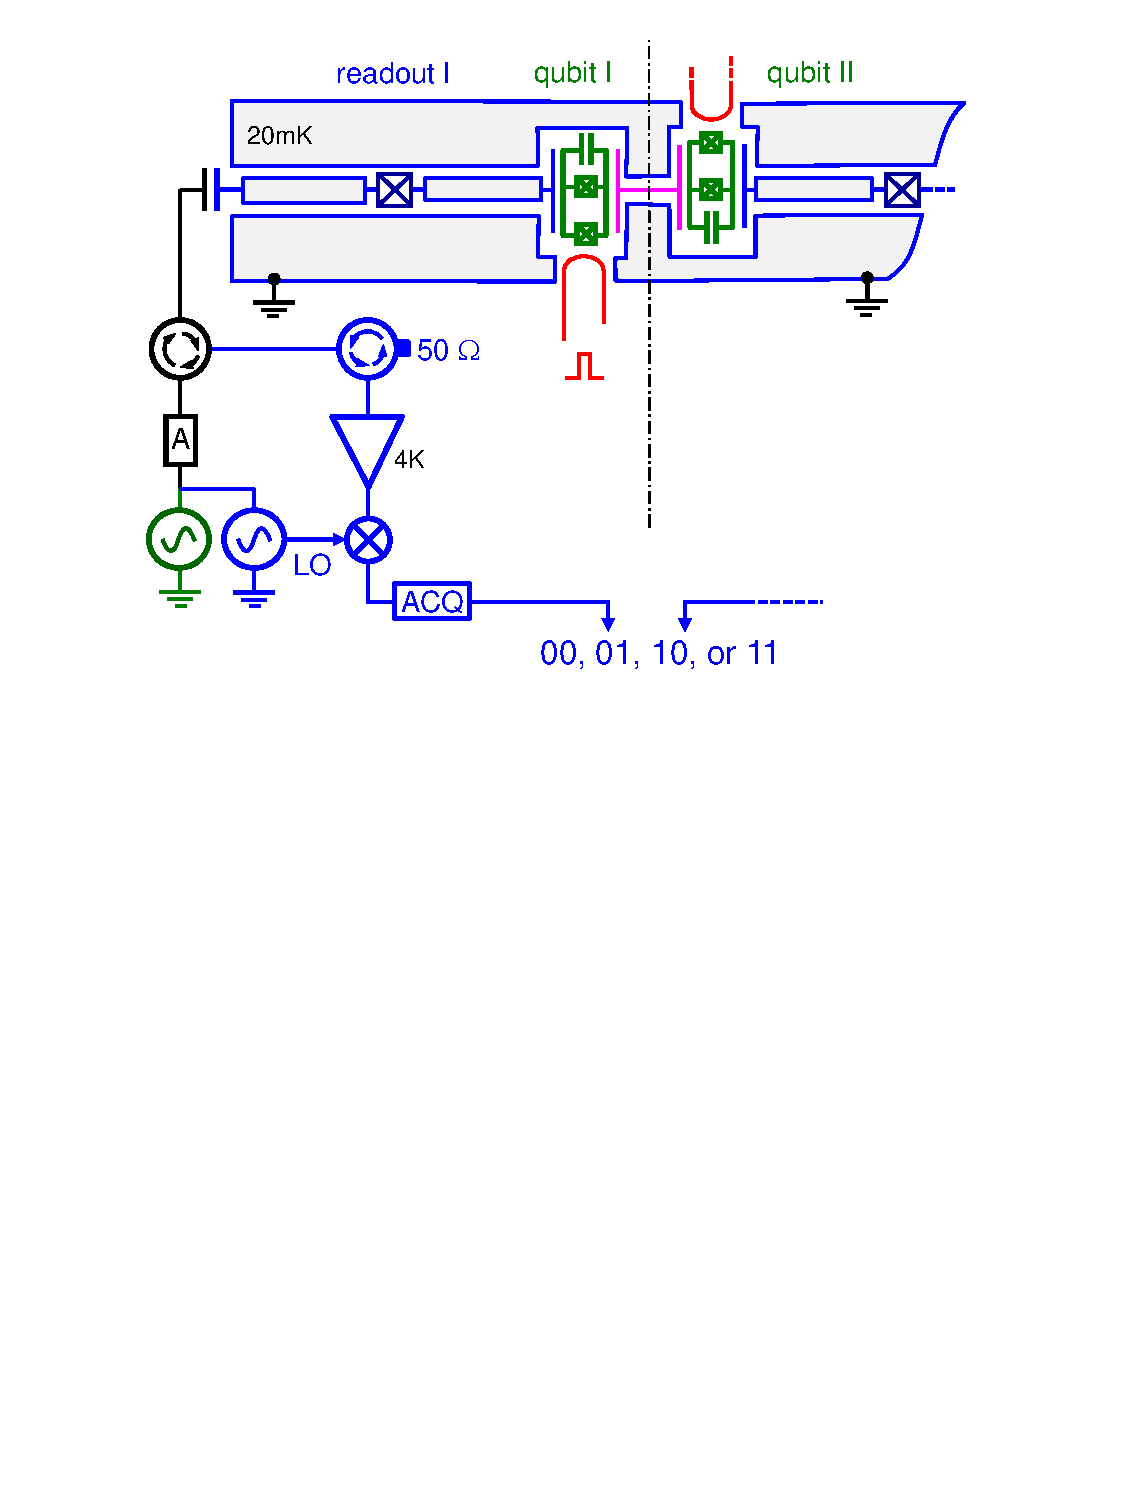
\includegraphics[width=0.75\textwidth]{./material/papers/grover/figures/2_qubit_processor_schematic}
	\caption[Circuit schematic of the realized two-qubit processor]{Circuit schematic of the two-qubit processor realized in this work, showing the two qubits in green, the qubit readouts in blue and the fast flux lines in red. Each qubit is embedded in its own nonlinear readout resonator and can be driven and read out through an individual microwave line.}
	\label{fig:two_qubit_processor_schematic}
\end{figure}

The quantum processor implemented in this work is shown in fig. \ref{fig:two_qubit_processor_schematic}. It consists of two superconducting quantum bits of the Transmon-type, each equipped with its own drive and readout circuit. The qubit readout is realized by using a nonlinear coplanar-waveguide resonator which serves as a cavity bifurcation amplifier (CBA)\citep{vijay_invited_2009} and implements a single-shot readout of the qubit state. Each qubit can be manipulated by driving it with microwave pulses through its readout resonator, allowing robust and fast single-qubit operations. The qubit frequencies can be tuned individually by fast flux lines, which allows to change the frequency each qubit over a range of several GHz. The coupling between the two qubits is realized through a fixed capacitance that connects the two top-electrodes of the qubits and implements a fixed $\sigma_{xx}$-type qubit-qubit coupling. This coupling allows us to implement a two-qubit gate and to generate entangled two-qubit states. We use this simple processor to test Bell's inequality, implement an universal two-qubit gate and perform a simple quantum algorithm that demonstrates probabilistic quantum speed-up, as will be discussed in the following sections.

\section{Demonstrating Simultaneous Single-Shot Readout}

\begin{figure}[ht!]
	\centering
		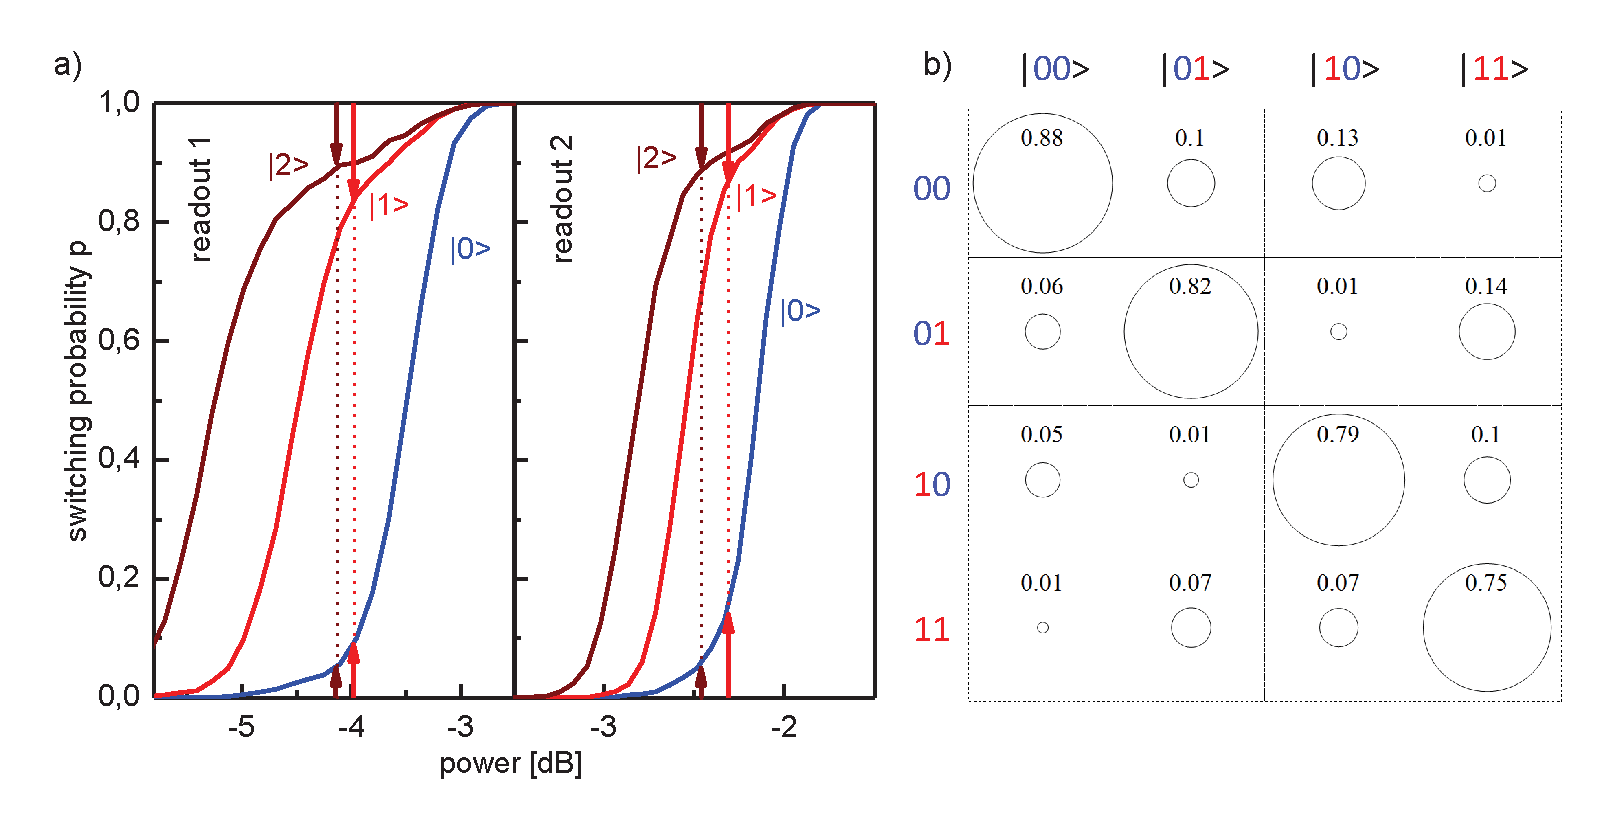
\includegraphics[width=1.\textwidth]{./material/papers/grover/figures/simultaneous_readout_characteristics}
	\caption[Switching probabilities of the two qubit readouts as a function of the readout excitation power]{a) Switching probabilities of the two qubit readouts as a function of the readout excitation power. The measurement is performed after preparing the qubits in the states $\color{blue}{\ket{0}}$, $\color{red}{\ket{1}}$ and $\color{brown}{\ket{2}}$. The readout fidelity is given as the difference in probability between the curves corresponding to the states $\color{blue}{\ket{0}}$ and $\color{red}{\ket{1}}$ or $\color{brown}{\ket{2}}$, respectively. The highest readout fidelites of 88 and 89 \% are achieved when the qubit is in state $\color{brown}{\ket{2}}$. b) Readout matrix of the two-qubit system. The matrix contains the probabilities of obtaining a given measurement result after having prepared the system in a given state. \figcomment{Replace this figure since it is not very intuitive. It would be better to show something which allows the reader to directly quantify the visibility and readout crosstalk present in the system.}}
	\label{fig:qubit_readout_characteristics}
\end{figure}

To read out the state of each qubit, a so-called cavity bifurcation amplifier \citep{siddiqi_dispersive_2006,mallet_single-shot_2009} is used. This readout technique works by capacitively coupling the qubit to a coplanar waveguide resonator which is rendered nonlinear by a Josephson junction placed in its center conductor. This nonlinear resonator can exhibit hysteretic behaviour for certain drive parameters, which can be used to map the state of the qubit to one of the bistable states of the resonator, thereby obtaining a single-shot readout. Contrary to other CQED approaches, in our setup each qubit is fitted with an individual CBA readout, allowing thus a simultaneous measurement of the full two-qubit register and therefore following closely the canonical blueprint of a quantum computer as formulated by DiVincenzo.\todo{discuss more details of the readout here...} Readout fidelitis up to 93 \% have been demonstrated using the CBA readout technique \citep{mallet_single-shot_2009} but due to design contraints only  83-85 \% fidelity have been attained in our experiments. The full characterization of the two-qubit readout is shown in fig. \ref{fig:qubit_readout_characteristics}. Fig. \ref{fig:qubit_readout_characteristics}a shows the so-called s curves of each qubit readout, which shown the working-point dependent switching probabilities of each readout with the qubits in different states. Fig. \ref{fig:qubit_readout_characteristics}b shows the full readout matrix, which connects readout switching probabilities with qubit state occupation probabilities and allows for the correction of all readout errors.

\section{Generating and Characterizing Entanglement}

\begin{figure}
	\centering
		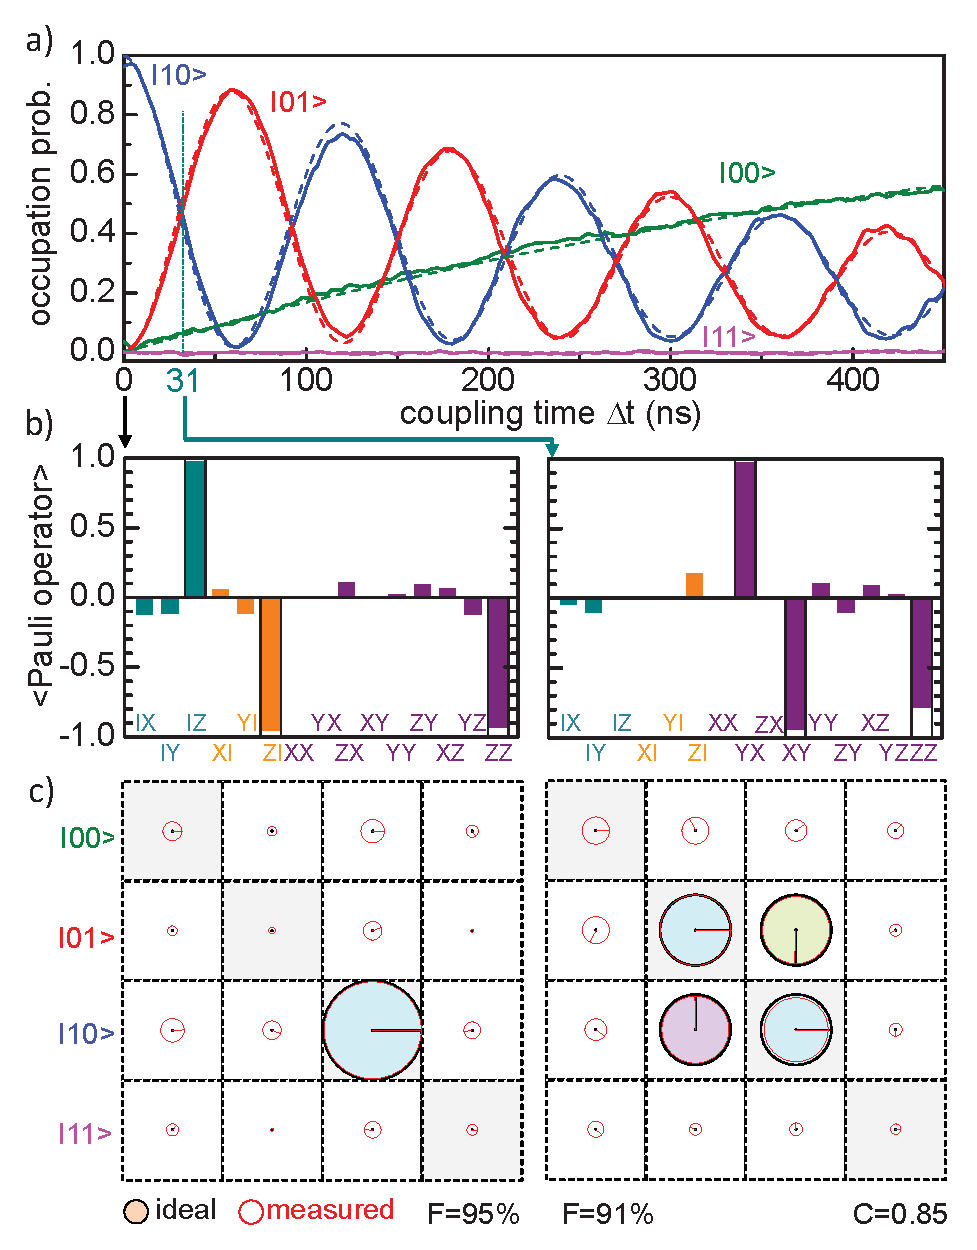
\includegraphics[width=0.7\textwidth]{./material/papers/iswap/submission1/Dewes_Figure2}
	\caption[Generating entangled two-qubit states by swapping interaction]{Energy oscillations between the two qubits induced by a resonant swapping interaction between them. a) The qubit state after switching on the swapping interaction for a given time $\Delta t$. The frequency of the oscillations corresponds to $2g = 8.7 \; \mathrm{MHz}$. b) The Pauli set of the two-qubit state measured at $0\; \mathrm{ns}$ and $31\; \mathrm{ns}$. c) The reconstructed density matrices corresponding to the two measured Pauli sets. In c), the area of each circle corresponds to the absolute value of each matrix element and the color and direction of the arrow give the phase of each element. The black circles correspond to the density matrices of the ideal states $\ket{10}$ and $1/\sqrt{2}/(\ket{10}+i\ket{01})$, respectively.\figcomment{verify sign!}}
	\label{fig:swap_interaction_state_tomography}
\end{figure}

The fixed coupling between the two qubits provides a $\sigma_{xx}$-type coupling which is only effective when the qubit frequencies are nearly resonant. Therefore, it can be switched on and off by changing the qubit frequencies, which we use to implement two-qubit gates with this system. In our processor, the effective coupling constant $g$ of the two qubits is given as $2g = 8.2 \; \mathrm{MHz}$\todo{Check if this is really $2g$!}. When using a fast fluxline pulse to abruptly tune the qubits in resonance we can switch on the qubit-qubit coupling non-adiabatically and generate an evolution operator of the form

\begin{equation}
	U(t)  =  \left( \begin{array}{cccc} 1 & 0 & 0 & 0 \\ 0 & \cos{2 \pi t g} & i\sin{2 \pi t g} & 0 \\ 0 & i\sin{2 \pi t g} & \cos{2 \pi t g} & 0 \\ 0 & 0 & 0 & 1 \end{array} \right) \label{eq:swap_evolution_operator}
\end{equation}

%explain that we stop the evolution at the right time to generate entangled states and implement a Two-qubit gate.

Switching off this interaction after a time $t_{\pi/2} = 1/8 g$ allows the creation of entangled qubit states and the implementation of a universal quantum gate, as will be explained later. Before doing this, we characterize the evoluation of the qubits during the swapping interaction by preparing them in the state $\ket{10}$, switching on the interaction for a given amount of time and measuring the qubit state directly afterwards. The resulting curve shown in fig. \ref{fig:swap_interaction_state_tomography} shows energy oscillations between the two qubits. Stopping the interaction after quarter of a period we obtain an entangled two-qubit Bell-type state that we can characterize by performing quantum state tomography. The experimental reconstruction of the density matrix of such a state corresponding approximating to the Bell-state $\ket{\psi} = 1/\sqrt{2}(\ket{01}+i\ket{10})$ is shown in fig. \ref{fig:swap_interaction_state_tomography}b. The measured fidelity of this state of 91 \% and the concurrence of 85 \% confirms that entanglement is present in the system. This entanglement can also be characterized by measuring the so-called {\it Clauser-Horne-Shimony-Holt} operator \citep{clauser_proposed_1969} on the produced state. This operator is given as

\begin{equation}
\mathrm{CHSH} = \mathrm{QS}+\mathrm{RS}+\mathrm{RT}-\mathrm{QT}
\end{equation}
with the operators $\mathrm{Q,R,S,T}$ being given as

\begin{eqnarray}
	\begin{array}{cccccccc}
		\mathrm{Q} & = & \sigma_z^1 &&& \mathrm{S} & = & \sigma_z^2\cdot \cos{\phi}+\sigma_x^2 \cdot \sin{\phi} \\
		\mathrm{R} & = & \sigma_x^1 &&& \mathrm{T} & = & -\sigma_z^2\cdot \sin{\phi}+\sigma_x^2 \cdot \cos{\phi}
	\end{array}
\end{eqnarray} 
Here, the angle $\phi$ is a parameter that should be chosen in accordance to the phase of the Bell state on which the operator is applied.

\begin{figure}[ht!]
	\centering
		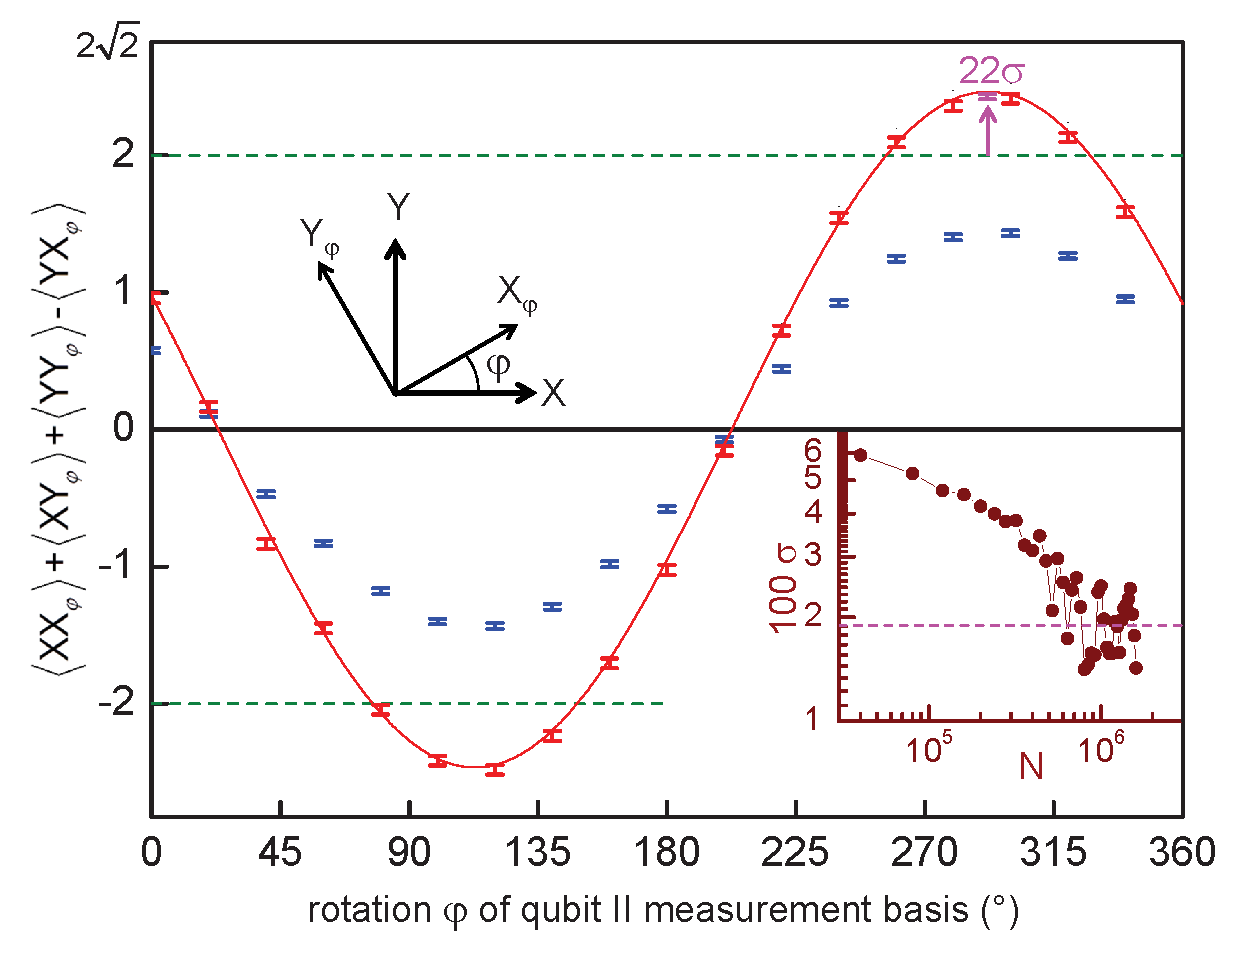
\includegraphics[width=0.7\textwidth]{./material/papers/iswap/submission1/Dewes_Figure3}
	\caption[Measurement of the CHSH operator of an entanged two-qubit state]{Measurement of the CHSH equation for an entangled two-qubit state. The renormalized CHSH expectation value (red points) exceeds the classical boundary of $2$ by a large amount. The raw measurement data (blue points) lies below this critical threshold. The inset shows the standard deviation $\sigma$ at the highest point of the curve as a function of the measurement sample size. For the highest sample count, the classical boundary is exceeded by $22$ standard deviations.\figcomment{p. 140 in cavities 6 labbook}}
	\label{fig:chsh_measurement}
\end{figure}

The expectation value $\bracket{CHSH}$ provides a test of the quantum-mechanical character of the generated state. For classical states, the maximum value is $\le 2$ but for entangled states it can reach a maximum value of $\sqrt{2}\cdot 2$. The result of a CHSH-type measurement performed on a state created by the method described above is shown in fig. \ref{fig:chsh_measurement}, showing the value of $\bracket{CHSH}$ as a function of $\phi$. We observe a violation of the classical boundary $2$ of the operator by $22$ standard deviations when correcting readout errors present in our system. However, the raw, uncorrected data fails to exceed the non-classical bound, making it impossible to close the detection loophole with our system. Nevertheless the observed violation of the equation by the renormalized state is a strong indication of entanglement in the system.

\section{Realizing a Universal Two-Qubit Quantum Gate}

\begin{SCfigure}[][ht!]
		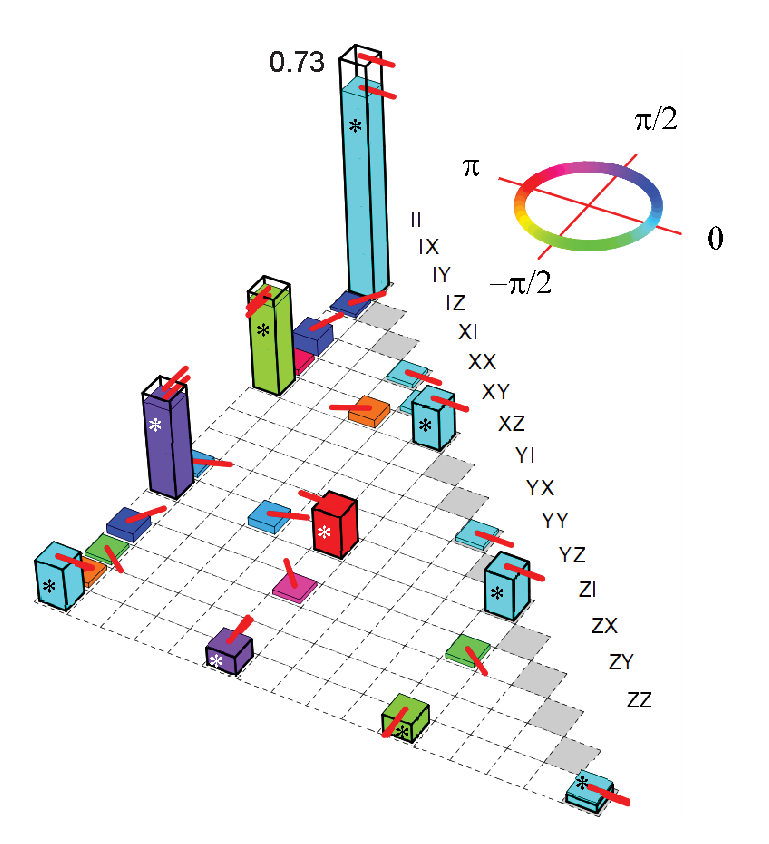
\includegraphics[width=0.65\textwidth]{./material/papers/iswap/figures/chi_matrix}
	\caption[Measured $\chi$-matrix of the $\sqrt{i\textrm{SWAP}}$ gate]{The measured $\chi$-matrix of the implemented $\sqrt{i\mathrm{SWAP}}$ gate. The row labels correspond to the indices of the $E_i$ operators, the height of each bar to the absolute value of the corresponding matrix element and the color and direction of the red arrow to the complex phase of each element. The ideal $\chi$-matrix of the $i\sqrt{\mathrm{SWAP}}$ gate is given by the outlined bars. The upper half of the positive-hermitian matrix is not shown.}
	\label{fig:gate_chi_matrix_and_errors}
\end{SCfigure}

The swapping evolution according to eq. (\ref{eq:swap_evolution_operator}) allows the implementation of a two-qubit gate. When switching on this interaction for $t_{\pi/2} = 1/8g$ we can realize the so-called $\sqrt{i\mathrm{SWAP}}$ gate, which has the representation

\begin{equation}
	\sqrt{i\mathrm{SWAP}}  =  \left( \begin{array}{cccc} 1 & 0 & 0 & 0 \\ 0 & 1/\sqrt{2} & i/\sqrt{2} & 0 \\ 0 & i/\sqrt{2} & 1/\sqrt{2} & 0 \\ 0 & 0 & 0 & 1 \end{array} \right) \label{eq:sqrt_iswap_gate}
\end{equation}
and is a universal two-qubit quantum gate. The operation and errors of our implementation of this gate can be characterized by performing quantum process tomography, yielding a gate fidelity of 90 \% . The 10 \% error in gate fidelity is caused mainly by qubit relaxation and dephasing during the gate operation and only marginally by deterministic preparation errors, as will be discussed in the main text of the thesis. Fig. \ref{fig:gate_chi_matrix_and_errors} show the measured $\chi$ matrix of the implemented gate. The achieved fidelity of the gate operation is sufficient to allow the implementation of a simple quantum algorithm with our processor, as will be discussed in the following section.
 
\section{Running a Quantum-Search Algorithm}

\begin{figure}[ht!]
	\centering
		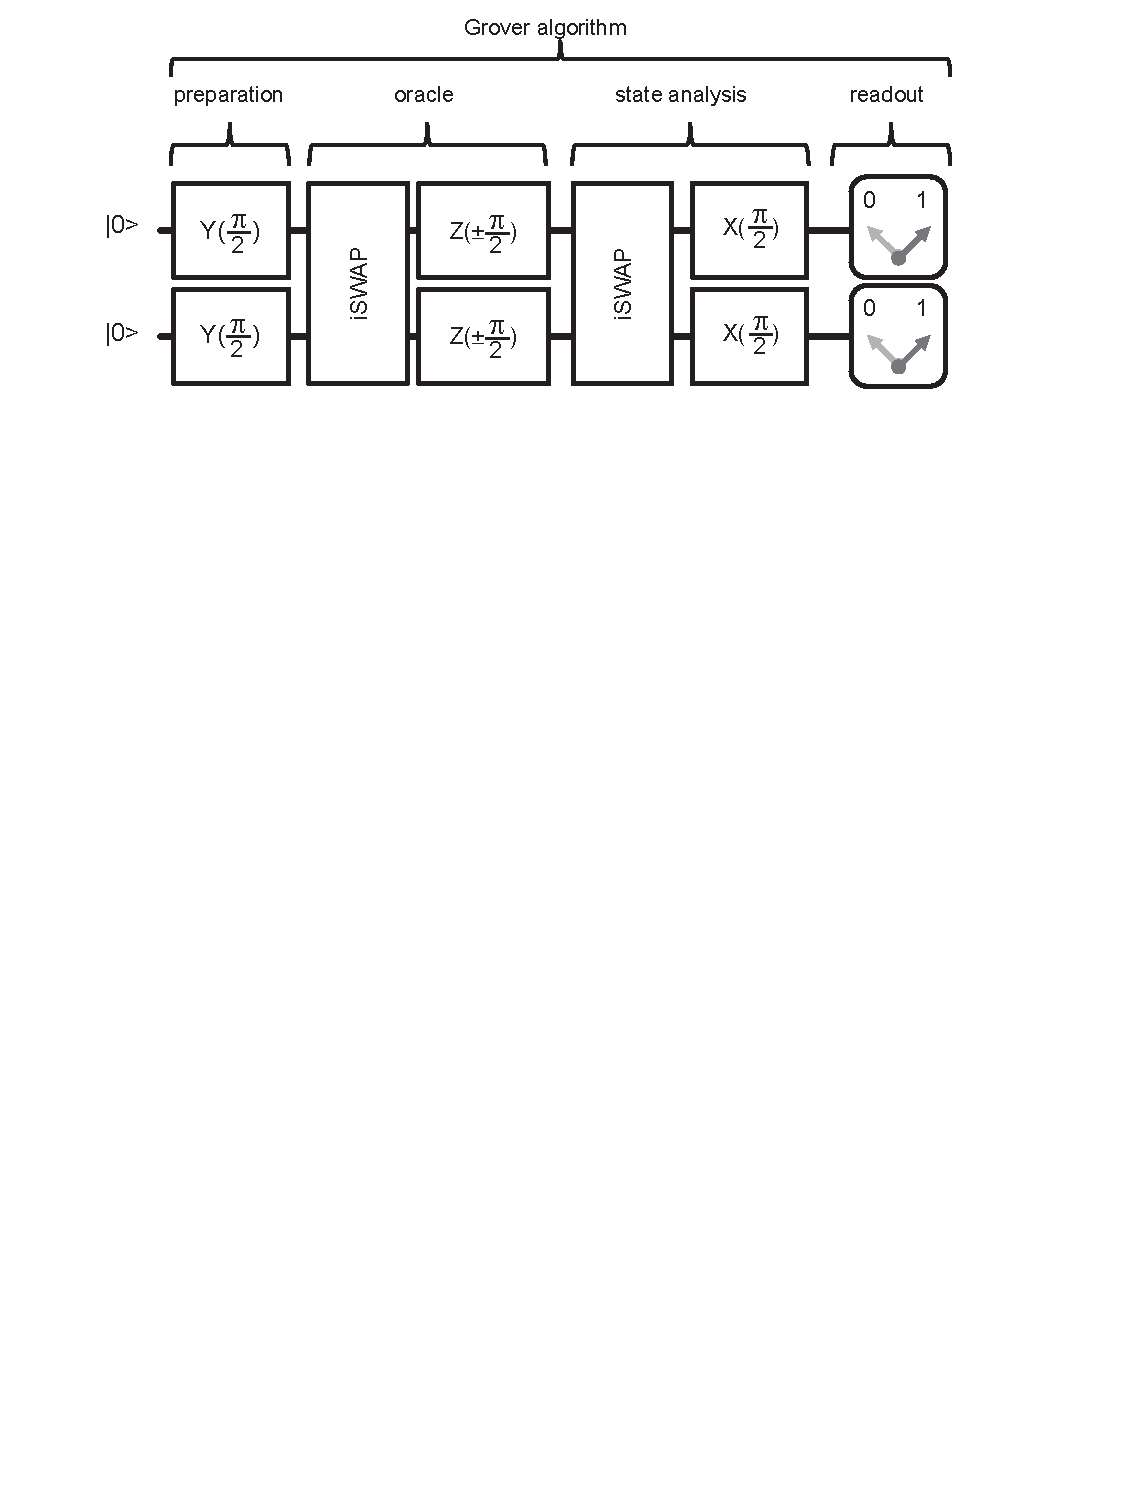
\includegraphics[width=0.8\textwidth]{./material/papers/grover/figures/grover_algorithm_schematic}
	\caption[Schematic of the implementation of Grovers search algorithm]{Schematic of the implementation of Grovers search algorithm on a two-qubit quantum processor. The algorithm consists in preparing a probe state, applying the quantum oracle to this state and analyzing the resulting output state to extract the information on the oracle operator.} 
	\label{fig:grover_algorithm_schematic}
\end{figure}

In this work we use the quantum gate implemented above to run a compiled version of Grover's search algorithm \citep{Grover_Quantum_1997}. The implemented version of the algorithm works in the basis of two qubits $x_i \in \{\ket{00},\ket{01},\ket{10},\ket{11}\}$ and  can distinguish between four different {\it oracle functions} $f(x)$ that each tag on one of the basis states $x_j$. Since the Grover algorithm for 2 qubits requires only one evaluation of the function $f(x)$ to determine which state has been marked it is faster than any conceivable classical algorithm, thus demonstrating the concept of quantum speed-up. The schematic of our version of Grover's algorithm is shown in fig. \ref{fig:grover_algorithm_schematic} and involves two $i\mathrm{SWAP}$ gates and three single-qubit operations along with a single-shot qubit readout at the end of the algorithm. We implemented all steps of this algorithm with our two-qubit processor and performed quantum state tomography after each step to reconstruct the quantum state at different points in the algorithm. Fig. \ref{fig:grover_density_matrices_state_1} shows the experimentially measured density matrices when running the algorithm with an oracle that marks the state $\ket{00}$. State tomographies are shown after applying the generalized Hadamard transform, after applying the quantum oracle and after the final step of the algorithm. This reconstruction of the quantum state using quantum state tomography does not however allow to demonstrate quantum speed-up, which requires individual single-shot readout of the qubit register, which will be discussed in the following section.

\begin{figure}[ht!]
	\centering
		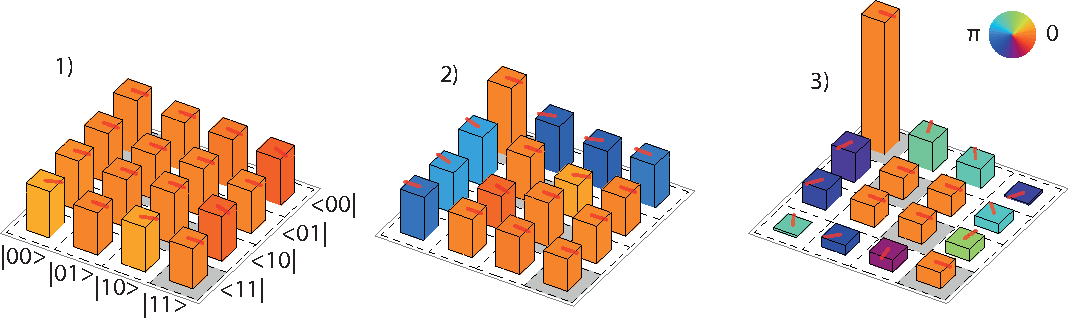
\includegraphics[width=1.\textwidth]{./material/figures/2-qubit-processor/grover/grover-density-matrices-state-1}
	\caption[Measured density matrices when running Grover's algorithm]{Measured density matrices when running Grover's search algorithm with a search oracle marking the state $\ket{00}$. 1) shows the state after the generalized Hadamard transform, 2) after applying the quantum oracle and 3) after the final step of Grover's algorithm.} 
	\label{fig:grover_density_matrices_state_1}
\end{figure}


\section{Demonstrating Quantum Speed-Up}

The main interest of running a quantum algorithm is to obtain an advantage in the run-time in comparision with a classical algorithm, the so-called {\it quantum speed-up}. To characterize this quantum speed-up as obtained with our processor, we run Grovers algorithm for all four possible oracle functions and directly readout out the qubit state after the last step of the algorithm, without correcting any readout errors. When averaging the results of such individual runs of the algorithm we can then obtain its single-run fidelity, which --for our processor-- ranges between 52 and 67 \%, depending on the state which is  marked by the quantum oracle, as shown in fig. \ref{fig:grover_single_shot_probabilities}. These results clearly demonstrate quantum speed-up in this system, although the achieved success probability is considerably lower than the theoretically possible value of 100 \% . The reduced fidelity is mainly due to relaxation and decoherence of the qubit state during the running of the algorithm and to a very small degree due to errors in the pulse sequence and drifts in the measurement equipment.

\begin{figure}[ht!]
		\centering
		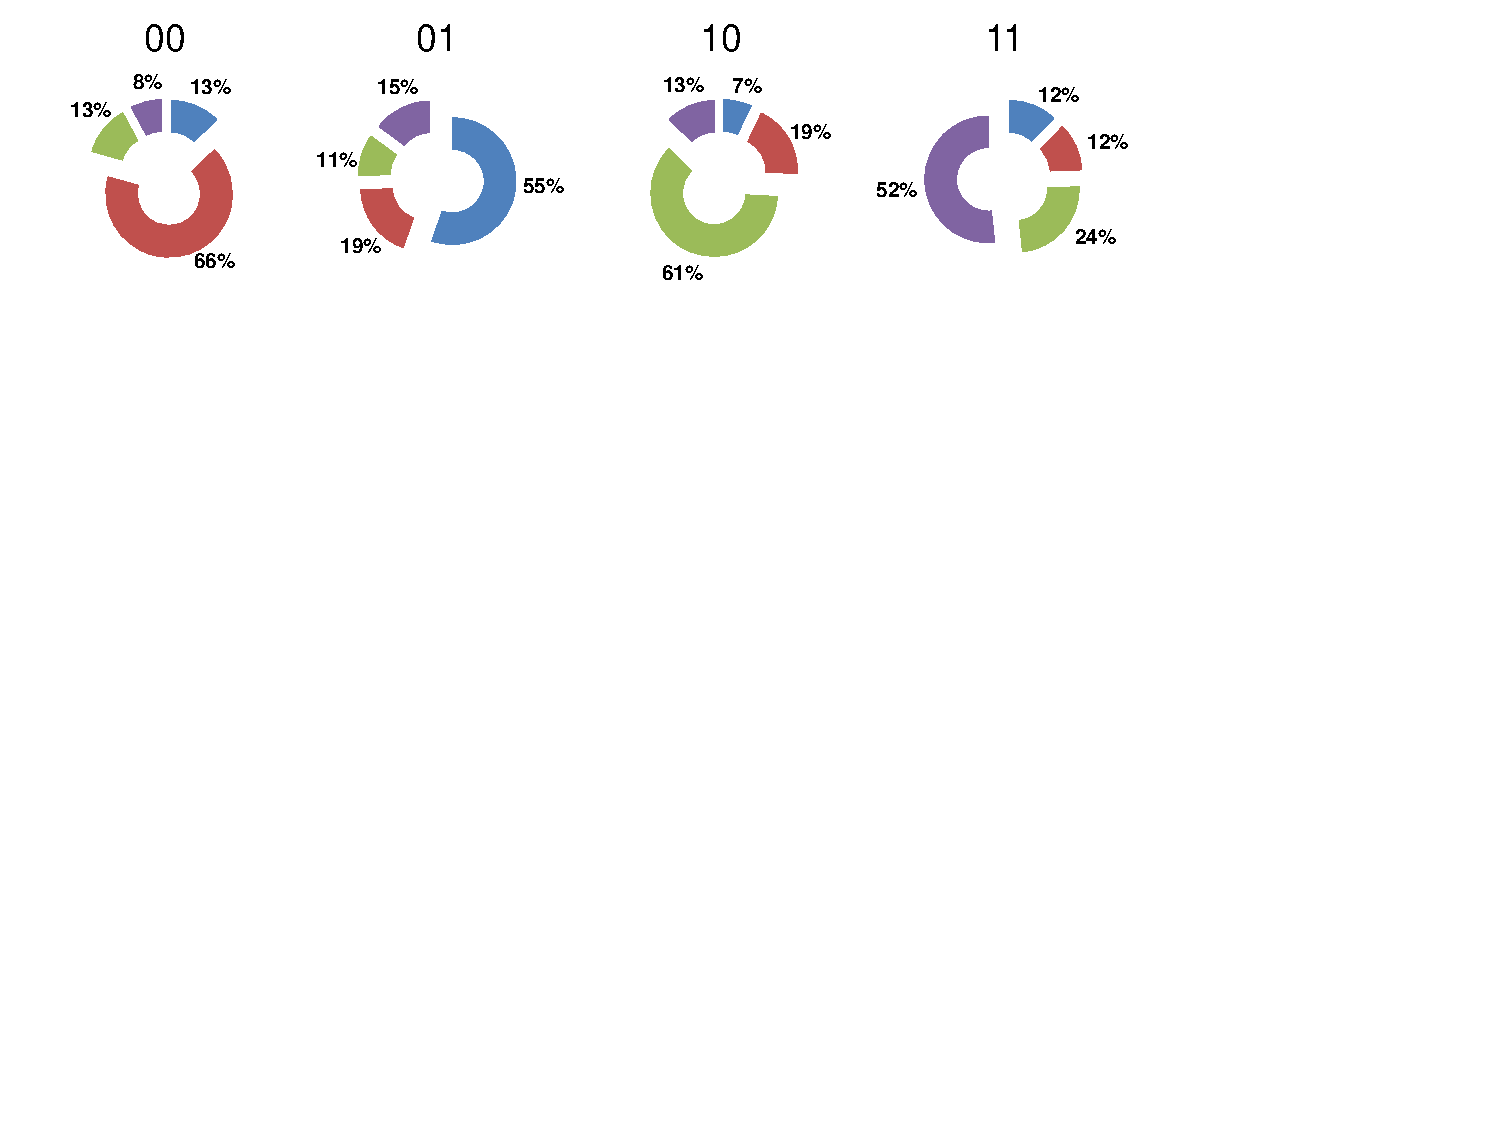
\includegraphics[width=1.0\textwidth]{./material/papers/grover/figures/grover_algorithm_single_shot_probabilities}
	\caption[Single-run results of the Grover search algorithm]{Single-run results when running the Grover search algorithm on our two-qubit quantum processor. Shown are the probabilities of obtaining the results $00,01,10,11$ as a function of the oracle function provided to the algorithm, indicated by the number on top of each graph. In all four cases, the success probability of the algorithm is $> 50 \%$, thus outperforming any classical algorithm in the number of calls to the oracle function.}
	\label{fig:grover_single_shot_probabilities}
\end{figure}

\section{Designing a Scalable Quantum Computing Architecture}

After having demonstrated the different building blocks of a superconducting, Transmon-based quantum processor it remains to be shown that larger-scale quantum-computing beyond two qubits is possible with this system. This work therefore pursued the realization of a more scalable qubit architecture using systems of up to six qubits coupled through a so-called ``quantum bus'' \citep{majer_coupling_2007}. The details of this novel architecture are discussed in the following sections.

The approach for scalable quantum computing with superconducting qubits pursued in this work consists of a system of many individual Transmon qubits equipped with individual JBA-based readouts, a multiplexed drive and readout circuit and a fixed qubit-qubit coupling mediated through a high-Q CPW resonator. As before, each qubit possesses a fluxline for fast frequency control. The readout and drive signals are send to all the qubits in parallel through a multiplexed transmission line. In this approach, the qubit and readout parameters, couplings and frequencies have to be carefully to avoid unwanted coupling between individual qubits and readouts and to allow the implementation of robust quantum gates between individual qubits. In this work we realized a 4-qubit chip and characterized it experimentally. The results of these experiments will be discussed in the main text of this thesis.

\begin{figure}[ht!]
  \centering
	\includegraphics[width=1.\textwidth]{"./material/figures/scalable-architecture/scalable architecture - schematic"}
	\caption[...]{...}
\end{figure}


\chapter{Theoretical Foundations} \label{chapter:theory}

In this chapter we provide the reader with the minimum conceptual background and theoretical building blocks necessary  to understand this thesis work. We begin our discussion with a general overview of classical and quantum information processing with a Turing machine, followed by an introduction to superconducting quantum circuits. We summarize the method to quantize electrical circuits and apply it to Cooper pair box devices, and in particular to the Transmon that will be used to implement the qubit register of our quantum processor. We then present coplanar waveguide resonators, and introduce circuit quantum electrodynamics on the example of a transmon coupled to a such a resonator. Finally, we consider the case of a nonlinear resonator used as a Josephson bifurcation amplifier since we use such a readout device in our processor architecture.

\section{Classical \& Quantum Information Processing}

\begin{SCfigure}
	\includegraphics[width=8cm]{"./material/figures/introduction/bloch_sphere"}
	\caption{The Bloch sphere representation of a qubit state $\ket{\psi} = \cos{\frac{\theta}{2}}\ket{0}+e^{i\phi}\sin{\frac{\theta}{2}}\ket{1}$. The state $\ket{\psi}$ is fully characterized by specifying its ``latitude'' and ``azimuth'' angles $\theta$ and $\phi$. Pure quantum states will always lie on the surface of the Bloch sphere, whereas mixed quantum states can also lie anywhere inside the sphere.}
	\label{fig:BlochSphere}
\end{SCfigure}

By definition, computing designates the activity of using computer hardware and software to process information, or {\it data}. Classical information processing can be divided in so-called {\it analog and digital information processing}, the former being based on continuously changeable physical quantities whereas the latter is based on incrementally changeable quantities. The fundamental unit of digital information processing is the so-called {\it bit}, which represents a Boolean (true/false) information. The discipline of theoretical computer science has been created to investigate the fundamental limits and properties of classical information processing. One of the main foundational theorems of theoretical computer science is the so-called {\it Church-Turing thesis} which provides a universal computing model by saying (basically) that everything which is computable can be efficiently computed using a {\it Turing machine}. Such a Turing machine, in turn, is a simple theoretical device which is able to run programs that operate on a discrete set of data using a well-specified set of operations. The Turing machine is universal in the sense that any other classical computing device can be efficiently emulated using a Turing machine with the appropriate program and data.

\smallskip

In the early 1980, Richard Feynman discovered that a classical Turing machine as described above would be unable to efficiently simulate a quantum-mechanical system \citep{feynman_simulating_1982}. He introduced the concept of a {\it quantum Turing machine} that would be able to simulate quantum-mechanical systems in an efficient manner. A few years later, David Deutsch took up Feynman's idea and developed an information processing framework based on quantum mechanics \citep{deutsch_quantum_1985}, coining the terms {\it quantum computing} and {\it quantum information processing}. He showed that by making use of different properties of quantum mechanics, namely, the superposition principle and entanglement, one could solve certain mathematical problems faster than possible with any classical computer \citep{deutsch_quantum_1985}. The work by Deutsch created a large interest in the physics community and led to a huge theoretical and experimental effort aimed at realizing an operational quantum computer and developing quantum algorithms for relevant real-world problems.

\section{Principles of "Conventional" Quantum Computing}

The first scheme imagined for quantum information processing is directly inspired from the classical digital Turing machine: information is stored in a set of quantum two level systems, the {\it quantum bits} or {\it qubits}, forming a quantum register, which is manipulated by sequentially applying unitary (and possibly non-unitary) operators to subsets of qubits in the register, typically one or two. As for a classical Turing machine, any arbitrary operation of this quantum processor can be decomposed as a sequence of gate operations chosen from a surprisingly small set of gates, said universal. The power of such a machine comes from the gates operating on superposed states, which provides an intrinsic parallelism in the processing.
\smallskip
This {\it quantum gate} approach is the method relevant to the present thesis work, and we ignore other approaches introduced more recently such as {\it one-way quantum computing} \citep{raussendorf_one-way_2001}, {\it adiabatic quantum computing} \citep{farhi_quantum_2000} or {\it topological quantum computing} \citep{kitaev_fault-tolerant_2003}. In this section we introduce very briefly quantum bits and quantum gates, as well as some examples of quantum algorithms that are relevant to this work.


\subsection{Quantum Bits and registers}

As in classical computing, one can define in quantum computing a fundamental unit of information: the qubit. Such a qubit is a quantum-mechanical two-level system that can be put in any superposition
%
\begin{equation}
\ket{\psi} = \cos{\frac{\theta}{2}}\ket{0}+e^{i\phi}\sin{\frac{\theta}{2}}\ket{1}
\end{equation}
%
of its two states $\ket{0}$ and $\ket{1}$.
As can be seen, any state can be described by a pair of real numbers $\theta$ and $\phi$ that characterize the amplitude of each of the two basis states and the phase between them. A useful and intuitive representation of such a single-qubit state is the so-called {\it Bloch sphere representation}, shown in fig. \ref{fig:BlochSphere}. The north and south poles of this sphere correspond by convention to the qubit states $\ket{0}$ and $\ket{1}$ (or vice versa). In this representation, any pure state $\ket{\psi}$ is located on a unit sphere. All states lying on the sphere between those two correspond to superposition states, which are characterized by their ``latitude'' and ``azimuth'' angles $\theta$ and $\phi$. 

\smallskip

\smallskip
If the qubit state is not pure but is a mixed state given by the complete set of probabilities ${p_{i}}$ to find it in one of the pure states  ${\ket{\psi_{i}}}$, it is characterized by the density matrix $\rho_{mixed} = \sum\limits_i p_i \rho_i$ with $\rho_i=\ket{\psi_{i}}\bra{\psi_{i}}$ the density matrix of the pure state $\ket{\psi_i}$. These $\rho$'s are Hermitian $2\times 2$ matrices with non-negative eigenvalues and can be written as
%
\begin{equation}
\rho = \left( \begin{array}{cc} \rho_{00} & \rho_{01} \\ \rho_{01}^* & \rho_{11} \end{array} \right),
\end{equation}
%
in the ${\ket{0},\ket{1}}$ basis, with $\rho_{00}$ and $\rho_{11}$ being real numbers and $\rho_{01}$ a complex number. For any state, the matrix has a unity trace $\mathrm{Tr}(\rho)=1$, for pure states we have $\rho=\rho^2$ in addition. The expectation values $\langle A \rangle$ of any operator $A$ acting on the density matrix $\rho$ is given as $\mathrm{Tr}(\rho A)$.

\smallskip

A mixed single-qubit state $\rho$ can also be represented on the Bloch sphere. For this, we decompose $\rho = c_i\sigma_I+c_x\sigma_x+c_y\sigma_y+c_z\sigma_z$, where $c_{i,x,y,z}$ are complex coefficients and the Pauli matrices $\sigma_I,\sigma_x,\sigma_y,\sigma_z$ are
%
\begin{align}
  \sigma_I  =  \left( \begin{array}{cc} 1 & 0 \\ 0 & 1 \end{array} \right)
 & &  \sigma_x  =  \left( \begin{array}{cc} 0 & 1 \\ 1 & 0 \end{array} \right)
  & & \sigma_y  =  \left( \begin{array}{cc} 0 & -i \\ i  &  0\end{array} \right)
  & & \sigma_z  =  \left( \begin{array}{cc} 1 & 0 \\ 0 & -1 \end{array} \right).
\label{eq:pauli_operators}
\end{align}
% 
We can then plot the vector $(c_x,c_y,c_z)$ in the Bloch sphere. The length of this vector decreases from 1 for a pure state down to 0 for a completely mixed state.

\smallskip

Quantum states with more than one qubit cannot be described anymore using Bloch spheres but are easily described with density matrices of dimension $2^n\otimes 2^n$ in the computational basis $\ket{q_1\hdots q_n}=\ket{q_1}\otimes\ket{q_{2}}\hdots\otimes\ket{q_n}$.For example, a two-qubit Bell state of the form $\ket{\psi_+}=(\ket{01}+\ket{10})/\sqrt{2}$ can be written as
%
\begin{equation}
\rho_{\psi_+} = \frac{1}{2}\left( \begin{array}{cccc} 0 & 0 & 0 & 0 \\ 0 & 1 & 1 & 0 \\ 0 & 1 & 1 & 0 \\ 0 & 0 & 0 & 0 \end{array} \right)_{(\ket{00},\ket{01},\ket{10},\ket{11})}
\end{equation}
%
whereas a completely mixed state of 50 \% $\ket{01}$ and 50 \% $\ket{10}$ is represented by the matrix
%
\begin{equation}
\rho_{\psi_+} = \frac{1}{2}\left( \begin{array}{cccc} 0 & 0 & 0 & 0 \\ 0 & 1 & 0 & 0 \\ 0 & 0 & 1 & 0 \\ 0 & 0 & 0 & 0 \end{array} \right)_{(\ket{00},\ket{01},\ket{10},\ket{11})}
\end{equation}
%

\subsection{Quantum Gates}

Analogously to classical information processing one defines {\it quantum gates} that act on individual or multiple qubits and allow us to process information. Such a quantum gate can be described as a unitary operator acting on a part of the Hilbert space representing the qubit register. Theoretically there is an infinite number of possible quantum gates, however in order to describe all possible quantum operations that can be performed on a qubit register of arbitrary length it is sufficient to defined a so-called {\it universal set of quantum gates}. Such a set contains a small number of quantum gates that can, by concatenation, produce any arbitrary unitary quantum operator, as shown by the so-called {\it Solovay-Kitaev theorem} \citep{nielsen_quantum_2000,dawson_solovay-kitaev_2005}. Such a universal gate set that will be especially relevant to this work consists of the three single-qubit rotation matrices
%
\begin{eqnarray}
   R_x(\theta)  & = & e^{-i\sigma_x\frac{\theta}{2}} \\ 
   R_y(\theta)  & = & e^{-i\sigma_y\frac{\theta}{2}} \\ 
   R_z(\theta)  & = & e^{-i\sigma_z\frac{\theta}{2}} 
\label{eq:universal_single_qubit_gates}
\end{eqnarray}
%
together with the so-called $\sqrt{i\mathrm{SWAP}}$
%
\begin{equation}
\sqrt{i\mathrm{SWAP}} = \left( \begin{array}{cccc} 1 & 0 & 0 & 0 \\ 0 & 1/\sqrt{2} & i/\sqrt{2} & 0 \\ 0 & i/\sqrt{2} & 1/\sqrt{2} & 0 \\ 0 & 0 & 0 & 1  \end{array}  \right)_{(\ket{00},\ket{01},\ket{10},\ket{11})}
\end{equation}
%
By applying the $\sqrt{i\mathrm{SWAP}}$ operation twice we obtain the $i\mathrm{SWAP}$ quantum gate, which is, by itself, \textbf{not} a universal quantum gate but which is nevertheless used in some practical quantum algorithms:
%
\begin{equation}
i\mathrm{SWAP} = \left( \begin{array}{cccc} 1 & 0 & 0 & 0 \\ 0 & 0 & i & 0 \\ 0 & i & 0 & 0 \\ 0 & 0 & 0 & 1  \end{array}  \right)_{(\ket{00},\ket{01},\ket{10},\ket{11})}
\end{equation}
%

This universal set it not minimal, since in principle two single-qubit gates with a fixed rotation angle (e.g. $R_x(\pi/4)$ and $R_y(\pi/4)$) together with a universal two-qubit gate would be sufficient to form a universal set of gates \citep{dawson_solovay-kitaev_2005}. However, it is often advantageous if one can use single-qubit rotations with arbitrary rotation angles around all three axes of the Bloch sphere since it can significantly reduce the number of gates required to implement a given unitary operation.

\subsection{Quantum Algorithms}

The interest in quantum computing is mainly due to the fact that certain problems can be solved faster on a quantum computer than on a classical computer. By faster we mean here that the order $\cal{O}$ of the run time of the algorithm increases faster on a classical computer than on a quantum computer as a function of the problem size, i.e. the number of bits needed to encode the problem. Up to this day it has not been demonstrated that a quantum computer can perform all tasks faster than a classical computer. However, a small number of real-world problems have been found that can be solved exponentially to polynomially faster on a quantum computer. Here we cite only the two most ``famous'' ones:

\begin{enumerate}
\item \textbf{The Shor Factorization Algorithm} Developed by Peter Shor in 1994 \citep{shor_algorithms_1994,shor_polynomial-time_1995}. This algorithm can factorize a binary number of length $N$ into its prime factors in $\begin{mathcal}O\end{mathcal}(\log^3{N})$ steps, therefore exponentially outperforming any known classical factorization algorithm. There is large interest in this algorithm since products of large prime numbers are routinely used in asymmetric cryptography.
\item \textbf{The Grover Search Algorithm}: Discovered by Lov Grover in 1996 \citep{grover_fast_1996}, this search algorithm can find a single well-defined state in an unsorted database of size $N$ in $\begin{mathcal}O\end{mathcal}(\sqrt{N})$ steps, being hence quadratically faster than a classical search algorithm (http://en.wikipedia.org/wiki/Quantum\_algorithm).
\end{enumerate}

\subsection{Quantum Simulation}

Another domain of interest for quantum computers is the so called {\it quantum simulation} \citep{lloyd_universal_1996}. Here the goal is to simulate the behavior of an arbitrary quantum system using a quantum computer by either engineering the quantum computer in direct analogy with the system being modeled (so called {\it analog quantum simulation}) or by numerically simulating the Hamiltonian of the quantum system on a general-purpose quantum computer (so-called {\it digital quantum simulation}). Since no classical computer can simulate a quantum system efficiently, there is a large interest in quantum simulation, especially in the fields of biology \& chemistry \citep{barreiro_open-system_2011}, quantum field theory \citep{gerritsma_quantum_2010,freedman_simulation_2002} and many-body physics \citep{simon_quantum_2011}.

\subsection{Realization of a Quantum Computer}

To realize a working quantum computer, it is necessary to implement highly coherent qubits that can be manipulated, read out and coupled with high fidelity. So far, no fully working quantum computer has been experimentally demonstrated. However, larger progress towards its realization has been achieved in the last decade. Promising approaches for its realization include, among others, ions trapped in magnetic and electric fields \citep{monroe_demonstration_1995,cirac_quantum_1995}, nuclear magnetic resonance of organic molecules \citep{jones_nmr_2001,vandersypen_experimental_2001}, cold atomic gases \citep{briegel_quantum_2000}, photonic circuits \citep{knill_scheme_2001}, semiconductor circuits \citep{loss_quantum_1998} and, last but not least, superconducting circuits. Since this work treats only superconducting qubits, we focus our attention on them. We explain how we can realize a reliable qubit using superconducting structures and how we can implement circuits to manipulate, couple and read out the qubit state.

\section{Superconducting Quantum Circuits}

In this section we discuss several types of superconducting circuit elements that are most relevant to this work. First, we introduce the reader to the Josephson junction, which is the device we use to realize superconducting qubits and amplifiers. Then, we present a general method for the quantization of arbitrary electrical circuits that we use afterwards to perform canonical quantization of our circuits. We use this method to derive the Hamiltonian of the Cooper pair box and treat the Transmon qubit as a special case. Afterwards, we discuss the properties of transmission lines and transmission line resonators that we use extensively for implementing readout and coupling elements in our qubit design. Then we give a short overview of the field of circuit quantum electrodynamics and finally introduce the reader to the Josephson and cavity bifurcation amplifiers that we use for our qubit readout.

\subsection{The Josephson junction}

The core element used to construct quantum circuits is the so-called {\it Josephson junction}, being equivalent in significance to the transistor in classical circuits. A Josephson junction is based on the so-called Josephson effect \citep{josephson_possible_1962}, which states that between two superconductors connected through an insulating barrier, a supercurrent
%
\begin{equation}
I = I_c\sin{\varphi}
\end{equation}
%
will flow, depending on the difference $\varphi = \varphi_2-\varphi_1$ between the gauge-invariant superconducting phases $\varphi_1$ and $\varphi_2$ at each side of the link. $I_c$ is the so-called {\it critical current} of the Josephson junction, which is the maximum current that it can support without transitioning to a resistive state. $\varphi$ is related to the instantaneous voltage between the electrodes of the junction as
%
\begin{equation}
V = \varphi_0\frac{\partial \varphi}{\partial t},
\end{equation}
%
where $\varphi_0 =\hbar/2e \approx 3.26\times 10^{-16}\;\mathrm{Wb}$. These two simple equations yield a system exhibiting a  wealth of interesting physical phenomena which are used today in various applications such as quantum limited amplifiers \citep{vijay_invited_2009}, generation of Terahertz radiation \citep{ozyuzer_emission_2007} and voltage standards \citep{levinsen_inverse_1977}. The energy associated with the phase difference across the Josephson junction is
%
\begin{equation}
E = E_J\cdot(1-\cos{\varphi})
\end{equation}
%
where $E_J = I_c\varphi_0$ is the so-called {\it Josephson energy}. In addition to this Josephson energy, the junction usually has an electrostatic energy associated to its capacitance (formed by its two electrodes) given as $E_C = Q^2/2C$, with $\pm|Q|$ being the charge accumulated on each of the electrodes of the junction.

\smallskip

For currents $I\ll I_c$, the Josephson junction behaves approximately like a nonlinear inductance
%
\begin{equation}
L_J(\varphi) = \frac{\varphi_0}{I_c \cos{\varphi}} \approx L_{J0}\left[1+\frac{\varphi^2}{2}+\begin{mathcal}O\end{mathcal}(\varphi^4)\right],\label{eq:josephson_inductance}
\end{equation}
%
where $L_{J0}=\varphi_0/ I_c$ is the so-called {\it Josephson inductance}. 

\smallskip

Using the potential and capacitive energies of the Josephson junction, we can formulate the quantum Hamiltonian of the junction, which is
%
\begin{equation}
\hat{H} = \frac{1}{2C}\hat{Q}^2+E_J(1-\cos{\hat{\varphi}}),
\end{equation}
%
where $\hat{\varphi}$ and $\hat{Q}$ are now conjugate quantum operators that, in analogy to a classical pendulum, play the role of position and momentum for the Josephson junction. In the limit of small angles $\varphi$, the Hamiltonian becomes that of a quantum harmonic LC oscillator. The nonlinearity present in the system is a key ingredient for realizing a Josephson junction qubit since it makes it possible to drive transitions between the first two quantum states of the device without also exciting higher quantum states, as would be the case for a quantum harmonic oscillator.

\subsection{Quantization of Electrical Circuits}

In this section we outline a general method to treat arbitrary electrical circuits as the ones discussed before within the framework of quantum-mechanics, hence {\it quantizing} them. This introduction on circuit quantization presented in this chapter is based on an article by B. Yurke \citep{yurke_quantum_1984} and an article by M. Devoret \cite{devoret_quantum_1995}. A more specific example of circuit quantization can be found in \citep{burkard_multilevel_2004}.

\smallskip

An electrical circuit is fully characterized by the parameters of its elements and its topology. The latter can be described as a set of nodes $j$ connected by a number of branches $i$ formed by the circuit elements . In classical circuit theory, each branch is described by a voltage $V_i$ between its ends and a current $I_{i}$ flowing through it. The Kirchhoff laws demand that the sum of the branch voltages $V_i$ along any closed path in the circuit must be zero and that the sum of currents flowing in and out of each node must be zero. For quantization it is usually more convenient to replace voltages and currents with branch charges and fluxes that are defined as
%
\begin{eqnarray}
\Phi_i(t) & = & \int\limits_{-\infty}^t V_i(t') dt' ;\\
Q_i(t) & = & \int\limits_{-\infty}^t I_i(t') dt'.
\end{eqnarray}
%
The Kirchhoff laws now write
%
\begin{align}
\sum\limits_{i} Q_i  =  Q_c & & , & & \sum\limits_{i}\Phi_i = \Phi_c \label{eq:kirchhoff_charge}
\end{align}
%
where $Q_c$ and $\Phi_c$ are constants and where the first sum is over charges $Q_i$ of all elements connected to a certain node and the second one is over all branches forming a closed loop in the circuit. We can obtain a complete set of node and branch equations for any given circuit by constructing the so-called {\it spanning tree} of the circuit, which is a tree in which all nodes are connected to an arbitrarily chosen {\it ground node} by one unique path \citep{devoret_quantum_1995}. From the spanning tree we can obtain a complete set of branches and the corresponding Kirchoff equations for the fluxes $\Phi_i$ around them. Together with the set of Kirchhoff equations for the charges at each node, we can use this system of equations to eliminate unnecessary circuit variables and obtain a description of the circuit using a minimal set of degrees of freedom. Now, to quantize a circuit made up of non-dissipative elements we can follow the method given in \cite{yurke_quantum_1984}, writing the Lagrangian (using the reduced set of variables) as 
%
\begin{equation}
\begin{mathcal}L\end{mathcal}(\Phi_1,\hdots,\Phi_n,\dot{\Phi}_1,\hdots,\dot{\Phi}_n) = \sum\limits_i \begin{mathcal}V\end{mathcal}_i - \sum\limits_i \begin{mathcal}T\end{mathcal}_i \label{eq:circuit_lagrangian}
\end{equation}
%
where the sum $i$ runs over all circuit elements and $\begin{mathcal}V\end{mathcal}_i$ and $\begin{mathcal}T\end{mathcal}_i$ are the potential and kinetic energies associated to the $i$-th circuit element. Here, linear inductances contribute only to the potential energy as $\begin{mathcal}V\end{mathcal}_{L_i} = \Phi_i^2/2L_i$, whereas linear capacitances contribute only to the kinetic energy as $\begin{mathcal}T\end{mathcal}_{C_i}=C_i\dot{\Phi}_i^2/2$. Resistors can be described within the Lagrangian formalism by modeling them as semi-infinite transmission lines with a characteristic impedance matching their resistance \citep{yurke_quantum_1984}. We can also include general nonlinear capacitances and inductances that obey the relations $\dot{\Phi}=f_C(Q)$ and $\dot{Q}=g_L(\Phi)$ between their node flux and charge, and whose energies are given as
%
\begin{eqnarray}
E_C = \int\limits_0^Q f_C(Q)dQ \\
E_L = \int\limits_0^\Phi g_L(\Phi)d\Phi
\end{eqnarray}
%
A Josephson junction, for example, can be described as a nonlinear inductance with $g_L^{JJ}(\Phi)=I_c\sin{(\Phi/\varphi_0)}$, having an associated energy
%
\begin{equation}
E_L^{JJ} = \int\limits_0^\Phi I_c\sin{\left(\Phi/\varphi_0\right)}=E_J(1-\cos{\left[\frac{\Phi}{\varphi_0}\right]}),
\end{equation}
%
. Transmission lines can be quantized by a similar approach, as shown e.g. in \citep{yurke_quantum_1984}. Externally imposed charges and fluxes can be modeled as ``pre-charged'' capacitors and inductors with infinite charge or flux and infinite capacitance or inductance that get renormalized at the end of the quantization process \citep{devoret_quantum_1995}. Externally imposed voltages and currents can be treated like this as well by converting them to corresponding fluxes or charges. From the Lagrangian as given by eq. (\ref{eq:circuit_lagrangian}) we can obtain the classical equations of motion of the system by variation of the action
%
\begin{equation}
\frac{\partial}{\partial t}\left( \frac{\partial \begin{mathcal}L\end{mathcal}}{\partial\dot{\Phi}_i}\right)-\frac{\partial \begin{mathcal}L\end{mathcal}}{\partial \Phi_i} = 0
\end{equation}
%
For each flux $\Phi_i$ we obtain its canonically conjugate momentum $Q_i$ by the equation
%
\begin{equation}
Q_i = \frac{\partial \begin{mathcal}L\end{mathcal}}{\partial(\dot{\Phi}_i)}, \label{eq:canonical_momentum}
\end{equation}
%
where $\dot{\Phi}_i=d\Phi_i/dt$. Having obtained $\Phi_i$ and $Q_i$, we can calculate the Hamiltonian $\begin{mathcal}H\end{mathcal}$ of the system by applying the transformation
%
\begin{equation}
\begin{mathcal}H\end{mathcal}(\Phi_1,\hdots,\Phi_n,Q_1,\hdots,Q_n) = \sum\limits_j \dot{\Phi}_i Q_i - \begin{mathcal}L\end{mathcal}(\Phi_1,\hdots,\Phi_n,\dot{\Phi}_1,\hdots,\dot{\Phi}_n) \label{eq:l_to_h}
\end{equation}
%
This Hamiltonian, written in generalized coordinates, yields the full set of equations of motion of the electrical circuit and depends only on the canonically conjugate variables $\Phi_{1},\hdots,\Phi_n$ and $Q_1,\hdots,Q_n$. First Quantization of the circuit can then be done by simply replacing the classical variables by quantum observables such that $\Phi_i\to\hat{\Phi}_i$ and $Q_i\to\hat{Q}_i$ and imposing commutation relations between them:
%
\begin{eqnarray}
\left[\hat{Q}_i,\hat{Q}_j\right] & = & 0 \\
\left[\hat{\Phi}_i,\hat{\Phi}_j \right] & = & 0 \\
\left[\hat{\Phi}_i,\hat{Q}_i\right] & = & i\hbar\delta_{ij} \label{eq:quantization_commutation_relations}
\end{eqnarray}
%
As an example, in the next section we apply this quantization method to to so-called {\it Cooper pair box} circuit, which is highly relevant to this work.

\subsection{The Cooper Pair Box}

\begin{figure}
	\centering
	\includegraphics[width=\textwidth]{"./material/figures/introduction/cooper_pair_box"}
	\caption{a) The circuit schematic of a Cooper Pair Box (CPB). The device consists of a Josephson junction capacitively coupled to a voltage source. The extra capacitance of the Josephson junction is modeled by a capacitor $C_\Sigma$. Charges can accumulate on the island between the voltage source and the Josephson junction. b) A {\it split Cooper pair box}, where instead of one junction two of them are arranged in a loop. With this geometry it is possible to tune the effective Josephson energy of the circuit by changing the magnetic flux inside the junction loop. c) The schematic of a split CPB capacitively coupled to ground. This schematic corresponds most closely to the experimental CPB circuit that we use in this work.}
	\label{fig:cpb_circuit}
\end{figure}

The {\it Cooper pair box (CPB)} is a device containing a Josephson junction coupled to an input voltage source through a gate capacitance $C_g$, as shown in fig. \ref{fig:cpb_circuit}a. Often one also uses two junction in a loop instead of a single one, as shown in fig. \ref{fig:cpb_circuit}b, which allows one to tune the effective Josephson energy of the system by changing the flux inside the junction loop, as will be explained in more detail later. Finally, in our experimental setup one separates the ground electrode of the CPB capacitively from the ground, as shown in fig. \ref{fig:cpb_circuit}c. In this section we discuss only case (a), since as we will show, (b) can be mapped to the simpler circuit (a) and the topology of (c) is mathematically equivalent to that of (b). The simple CPB circuit \ref{fig:cpb_circuit}a consists of  three nodes (including ground) and two branches. The flux $\Phi_2$ is not independent since it is set by the voltage source $V_g$, so we can directly eliminate it from the equations. This leaves us with only one remaining active node $\Phi_1$. Using these definitions, the Lagrangian of the circuit is given as
%
\begin{equation}
\begin{mathcal}L\end{mathcal}=\frac{1}{2}C_\Sigma\dot{\Phi}_1^2+\frac{1}{2}C_g\left(\dot{\Phi}_1+V_g\right)^2-E_J\left(1-\cos{\phi_1}\right)
\end{equation}
%
where $\phi_1=\Phi_1/\varphi_0$ . The canonical momentum $Q_1$ associated to the flux $\Phi_1$ is given as
%
\begin{equation}
Q_1 = \frac{\partial \begin{mathcal}L\end{mathcal}}{\partial \dot{\Phi}_1} = C_J \dot{\Phi}_1+C_g(V_g+\dot{\Phi}_1) \label{eq:q_of_phi}
\end{equation}
%
From this, we can directly calculate the Hamiltonian by using eq. (\ref{eq:l_to_h}) and substituting $Q_1$ as given by eq. (\ref{eq:q_of_phi}) for $\dot{\Phi}_1$, which yields
%
\begin{equation}
\begin{mathcal}H\end{mathcal} = E_J\left(1-\cos{\phi_1}\right)+\frac{(Q_1-C_g V_g)^2}{2(C_J+C_g)}-\frac{1}{2}C_g V_g^2
\end{equation}
%
Quantization of the Hamiltonian is completed by replacing $Q_i\to \hat{Q}_i$ and $\phi_i\to\hat{\phi}_i$ and imposing the commutation relations given by eqs. (\ref{eq:quantization_commutation_relations}). If, in addition we introduce reduced operators for the charge $\hat{n}=\hat{Q}/2e$ and discard the energy stored in the voltage source (which is irrelevant). We then obtain the Hamiltonian of the Cooper pair box, as formulated e.g. in the thesis of V. Bouchiat \citep{bouchiat_quantum_1998},
%
\begin{equation}
\hat{H} = E_C \left( \hat{n} - n_g\right)^2-E_J \cos{\hat{\phi_1}}, \label{eq:cpb_hamiltonian}
\end{equation}
%
with $E_C = (2e)^2 / (C_J+C_g)$ the charging energy of the Cooper pair box and $n_g=C_g V_g /2e $ the reduced gate charge.

\smallskip

For the split Cooper pair box as shown in fig. \ref{fig:cpb_circuit}b, the treatment is slightly modified \citep{cottet_implementation_2002}. First of all, we write the Josephson energies of the two junctions as $E_{J1}=(1+d)E_J/2$ and $E_{J2}=(1-d)E_J/2$, where $d$ is the energy asymmetry between the junctions. When imposing an external phase $\phi_{ext}=2\pi\Phi_{ext}/\tilde{\Phi}_0$ in the loop, the potential energy of the two junctions can be written as
%
\begin{eqnarray}
\begin{mathcal}V\end{mathcal}_J & = & -\frac{E_J}{2}\left[(1+d)\cos{(\phi_1-\phi_{ext}/2)}+(1-d)\cos{(\phi_2+\phi_{ext}/2)} \right] \\
& = & -E_J\left[\cos{\phi_1}\cos{\frac{\phi_{ext}}{2}}+d\sin{\phi_1}\sin{\frac{\phi_{ext}}{2}}\right].
\end{eqnarray}
%
The remaining part of the quantization process proceeds as above, yielding a Hamiltonian of the split Cooper pair box of the form
%
\begin{equation}
\hat{H}_{split} = E_C(\hat{n}-n_g)^2-E_J\left[\cos{\hat{\phi}_1}\cos{\frac{\phi_{ext}}{2}}+d\sin{\hat{\phi}_1}\sin{\frac{\phi_{ext}}{2}}\right]
\end{equation}
%
This Hamiltonian can be recast in the form \citep{cottet_implementation_2002}
%
\begin{equation}
\hat{H}_{split} = E_C(\hat{n}-n_g)^2-E_J'(d,\phi_{ext})\cos{[\hat{\phi}_1+\gamma(\phi_{ext})]},
\end{equation}
%
where
%
\begin{eqnarray}
E_J'(d,\phi_{ext}) & = & E_J\sqrt{\frac{1+d^2+(1-d^2)\cos{\phi_{ext}}}{2}} \\
\tan{\gamma(\phi_{ext})} & = & -d\tan{\frac{\phi_{ext}}{2}}
\end{eqnarray}
%
It is therefore possible to map the Hamiltonian of the split CPB to that of the single-junction one by defining $\hat{\theta}\to\hat{\phi}_1+\gamma(\phi_{ext})$ and $E_J\to E_J'(d,\phi_{ext})$. 

Using the Hamiltonian defined in eq. (\ref{eq:cpb_hamiltonian}), we can calculate the wave function of the simple Cooper pair box. The variables $\hat{n}$ and $\hat{\theta}$ are conjugate such that $[\hat{\theta},\hat{n}]=i\hbar$, the corresponding wave function $\Psi_k(\theta) = \bracket{\theta,k}$ will therefore satisfy a Schrödinger equation of the form
%
\begin{equation}
E_k \Psi_k(\theta) = E_C(\frac{1}{i}\frac{\partial}{\partial \theta}-n_g)^2 \Psi_k(\theta) - E_J \cos{\left(\theta\right)}\Psi_k(\theta) \label{eq:cpb_schroedinger_equation}
\end{equation}
%
Since the potential $-E_J\cos{(\theta)}$ is $2\pi$ periodic, the solution will be of the form
%
\begin{equation}
\Psi_k(\theta) = \Psi_k(\theta+2\pi),
\end{equation}
%
which allows us to map eq. (\ref{eq:cpb_schroedinger_equation}) to the so-called {\it Mathieu  equation}
%
\begin{equation}
\frac{d^2y}{dx^2}+\left[a-2q\cos{(2x)}\right]y = 0
\end{equation}
%
The {\it Floquet theorem} states that all solutions to this equation can be written in the form
%
\begin{equation}
F(a,q,x) = \exp{\left(i\mu x\right)}P(a,q,x)
\end{equation}
%
and the most general solutions are\citep{cottet_implementation_2002}
%
\begin{equation}
\Psi_k(r,q,\theta) = \mcal{C}_1\exp{\left(i n_g \theta \right)}\mcal{M}_C\left(\frac{4E_k}{E_C},-\frac{2E_J}{E_C},\frac{\theta}{2}\right)+\mcal{C}_2\exp{\left(i n_g \theta \right)}\mcal{M}_S \left(\frac{4 E_k}{E_C},-\frac{2 E_J}{E_C},\frac{\theta}{2}\right)
\end{equation}
%
with 
%
\begin{equation}
E_k = \frac{E_C}{4}\mcal{M}_A \left(r_k,-\frac{2 E_J}{E_C} \right)
\end{equation}
%
Here, $\mcal{M}_C$, $\mcal{M}_S$ are the so-called {\it Mathieu functions} and $\mcal{M}_A$ corresponds to the eigenvalue of each solution. Following the convention in \citep{cottet_implementation_2002} we order the $E_k$ such that the energy increases with increasing $k$, yielding \citep{koch_charge-insensitive_2007}
%
\begin{eqnarray}
r_k(n_g) & = & \sum\limits_{l\pm 1}\left[\mathrm{int}(n_g+l/2)\mathrm{mod}\;2\right] \notag \\
&  & \times\left\{\mathrm{int}(n_g/2)+l(-1)^k[(k+1)\mathrm{div}\;2]\right\}
\end{eqnarray}
%

\begin{figure}[ht!]
	\includegraphics[width=\textwidth]{"./material/mathematica/cooper_pair_box_energies"}
	\caption{Energies of the first four energy levels of the Cooper pair box for different ratios $E_J/E_C$, plotted as a function of the gate charge $n_g$. As can be seen, for $E_J \gg E_C$, the charge-dispersion curve becomes almost completely flat.}
	\label{fig:CooperPairBoxEnergies}
\end{figure}

We denote the energy differences between individual energy level by $E_{ij} = E_j - E_i$. We also define the absolute and relative anharmonicities of the first two energy levels as $\alpha \equiv E_{12}-E_{01}$ and $\alpha_r \equiv \alpha / E_{01}$. An in-depth treatment of the Cooper pair box can be found in \citep{cottet_implementation_2002}. Using the basis states $\ket{i}$ of the CPB, we can rewrite its Hamiltonian in the form 
%
\begin{equation}
\hat{H} = \hbar\sum\limits_{i=0} \omega_i\ket{i}\bra{i},
\end{equation}
%
where $\hbar\omega_i$ is the energy associated to the i-th CPB state. Disregarding CPB levels $i \ge 2$, we can also formulate an approximate qubit Hamiltonian of the CPB of the form
%
\begin{equation}
\hat{H} = -\frac{\hbar\omega_{01}}{2}\hat{\sigma}_z, \label{eq:cpb_qubit_hamiltonian}
\end{equation}
%
where $\omega_{01}=\omega_1-\omega_0$ is the frequency of the transition $\ket{0}\to\ket{1}$.

\subsubsection{The Transmon Qubit}

The Transmon qubit as developed in Yale by R. Schoelkopf {\it et. al.} \cite{koch_charge-insensitive_2007,wallraff_strong_2004} is a Cooper pair box in the regime where $E_J \gg E_C$. As shown in fig. \ref{fig:CooperPairBoxEnergies}, in this regime the charge dispersion of the energy levels of the Cooper pair box becomes almost flat, thus rendering the transition frequency $E_{01}$ practically insensitive to the value of the gate charge $n_g$. This reduced sensitivity to charge noise is highly advantageous in experiments since it increases the coherence time of the qubit. However, when increasing the ratio $E_J/E_C$, we also reduce the anharmonicity $\alpha_r$ of the qubit, therefore limiting the speed of gate operations that can be realized with this system (driving errors related to weak anharmonicity will be discussed more thoroughly chapter \ref{chapter:processor_characterization}). In the limit $E_J \gg E_C$ these qubit anharmonicities are well approximated by $\alpha \simeq -E_C$ and $\alpha_r \simeq -(8 E_J / E_C)^{-1/2}$. However, $\alpha_r$ decreases only geometrically with $E_J/E_C$, whereas the sensitivity of the qubit to charge noise decreases exponentially with the ratio of Josephson and charging energy.

\subsubsection{Decoherence of the Transmon}

An in-depth derivation of the decoherence of the CPB and the Transmon can be found e.g. in \citep{cottet_implementation_2002,koch_charge-insensitive_2007}. Here, we give the relevant expressions that we use to estimate the coherence of the Transmon qubits in our quantum processor. Fundamentally, {\it relaxation} and {\it dephasing} are the relevant decoherence mechanisms of the qubit, each one characterized by relaxation and dephasing rates $\Gamma_1$ and $\Gamma_\phi$ and corresponding coherence times $T_1=\Gamma_1^{-1}$ and $T_\phi=\Gamma_\phi^{-1}$. Following the treatment by Cottet {\it et. al.} \citep{cottet_implementation_2002}, a perturbation of the CPB Hamiltonian can be written as $\delta \hat{H}_{\lambda,S}=-\hbar/2(\mathbf{\hat{D}}_\lambda\cdot\mathbf{\sigma})\delta \mathbf{\hat{\lambda}}_S$. In the operator $\mathbf{D}$ we can distinguish between transversal parts $\hat{\mathbf{D}}_{\lambda,\perp}$ that describe relaxation processes and longitudinal parts $\hat{\mathbf{D}}_{\lambda,z}$ that describe dephasing processes. For the relaxation processes,we can calculate the relaxation rate from the sensitivity $\hat{\mathbf{D}}_{\lambda,\perp}$ and spectral density of the noise channel $S_{\lambda}(\omega_{01})$ using Fermi's golden rule:
%
\begin{equation}
\Gamma^{rel}_{S,\lambda} = \frac{\pi}{2}|D_{\lambda,\perp}|^2 S_{\lambda}(\omega_{01})
\end{equation}
%
Similarly, for the dephasing processes $\hat{\mathbf{D}}_{\lambda,z}$ we can calculate the dephasing rates using the corresponding sensitivities and spectral densities as
%
\begin{equation}
\Gamma_{S,\lambda}^\phi = \pi D_{\lambda,z}^2 S_{\lambda}(\omega = 0),
\end{equation}
%
assuming that the noise is regular at low frequencies. In the following paragraphs, we will discuss the most important relaxation and dephasing mechanisms for the CPB.

\smallskip

The most relevant couplings for relaxation and dephasing through the charge and current/phase channels of the CPB are
%
\begin{eqnarray}
D_{n_g,z} & = & -2\frac{E_C}{\hbar}\left(\bra{1}\hat{n}\ket{1}-\bra{0}\hat{n}\ket{0}\right) \\
D_{\theta/2\pi,z} & = & \frac{2\pi\Phi_0}{\hbar}\left(\bra{1}\hat{I}\ket{1}-\bra{0}\hat{I}\ket{0}\right) \\
D_{n_g,\perp} & = & 4\frac{E_C}{\hbar}\left|\bra{0}\hat{n}\ket{1}\right| \\
D_{\theta/2\pi,\perp} & = & \frac{4\pi\Phi_0}{\hbar}\left|\bra{0}\hat{I}\ket{1}\right|.
\end{eqnarray}
%
In chapter \ref{chapter:design} we will calculate the resulting relaxation and dephasing rate for a real-world Transmon qubit coupled to various external control parameters through the charge and flux channels.

\subsection{The LCR Resonator}

\begin{SCfigure}[1][ht!]
	\centering
	\includegraphics[width=0.4\textwidth]{"./material/figures/introduction/lcr_resonator"}
	\caption[]{An $LCR$ resonator coupled to a voltage source through an input capacitance $C_{in}$.}
	\label{fig:lcr_resonator}
\end{SCfigure}

The $LCR$ resonator is the circuit element that forms the basis of our qubit readout. The schematic of a $LCR$ resonator coupled to a voltage source through an input capacitance $C_{in}$ is  shown in fig. \ref{fig:lcr_resonator}. The impedance of the resonator alone is
%
\begin{equation}
Z_{LCR} = \frac{1}{\frac{1}{R}+i\omega C - \frac{i}{\omega L}},
\end{equation}
%
yielding a resonance frequency $\omega_r = 1/\sqrt{LC}$ and an {\it internal quality factor} $Q_{int} = \omega_r R C$. To probe the resonator we couple it through a gate capacitance $C_{in}$ to an input transmission line with characteristic impedance $Z_0$. We can model the resulting circuit as a LCR resonator with a frequency-dependent, effective resistance
%
\begin{equation}
R' = \left(\frac{1}{R}+\frac{C_{in}^2 Z_0 \omega^2}{1+C_{in}^2 Z_0^2 \omega^2}\right)^{-1}
\end{equation}
%
The quality factor of this {\it loaded resonator} changes according to 
%
\begin{equation}
Q^{-1} = Q^{-1}_{int}+Q^{-1}_{ext}
\end{equation}
%
where $Q_{ext} \approx \omega_r C (1+C_{in}^2Z_0^2\omega_r^2)/C_{in}^2 Z_0\omega_r^2 \approx \omega_r C Z_{in}/(C_{in}Z_0 \omega_r)^2$. As can be seen, the external quality factor increases $\propto 1 / C_{in}^2$. 

\subsubsection{Quantization of the Resonator}

The Hamiltonian of the non-dissipative part of the LCR resonator is
%
\begin{equation}
H = \frac{1}{2C}Q^2+\frac{1}{2L}\Phi^2
\end{equation}
%
This Hamiltonian corresponds to that of a harmonic oscillator and can be quantized as
%
\begin{equation}
\hat{H} = \omega_r\hbar\left(\hat{a}^\dagger\hat{a}+\frac{1}{2}\right). \label{eq:lc_hamiltonian}
\end{equation}
%
Here, $\hat{a}^\dagger$ and $\hat{a}$ are so-called {\it creation and annihilation operators} that can be written in function of the flux $\hat{\Phi}$ and charge $\hat{Q}$ operators as
%
\begin{eqnarray}
\hat{a}^\dagger & = & \sqrt{\frac{1}{2\hbar L \omega_r}}\left(\hat{\Phi}+iL\omega_r \hat{Q}\right)\\
\hat{a} & = & \sqrt{\frac{1}{2\hbar L\omega_r}}\left( \hat{\Phi}-iL\omega_r \hat{Q}\right)
\end{eqnarray}
%
By inverting these relations we obtain the flux and charge operators $\hat{\Phi}$ and $\hat{Q}$. Taking their time derivative gives us the voltage and current operators $\hat{V}$ and $\hat{I}$. These four operators are
%
\begin{eqnarray}
\hat{\Phi} & = & \sqrt{\frac{\hbar}{2C\omega_r}}\left(\hat{a}^\dagger+\hat{a}\right) \\
\hat{Q} & = & i\sqrt{\frac{C\omega_r\hbar}{2}}\left(\hat{a}^\dagger-\hat{a}\right) \\
\hat{V} & = & \sqrt{\frac{\hbar\omega_r}{2C}}\left(\hat{a}^\dagger+\hat{a}\right) \\
\hat{I} & = & i\omega\sqrt{\frac{C\omega_r\hbar}{2}}\left(\hat{a}^\dagger-\hat{a}\right)
\end{eqnarray}
%

\subsubsection{Coplanar Waveguide Resonators}

\begin{SCfigure}[1][ht!]
	\includegraphics[width=10cm]{"./material/mathematica/cpw_lambda_over_4_phase_and_z_with_schematic"}
	\caption{a) The electric field $E$ and current $I$ inside a $\lambda/2$ resonator. b) The circuit model of an open $\lambda/2$ resonator capacitively coupled to a drive circuit. The resonator can be modeled as a series of infinetesimal sections of $LC$ elements, as shown in the inset. c) The schematic of a coplanar waveguide (CPW) resonator, showing the electric field $E$, magnetic field $B$ and the current $I$ in the resonator. d) The reflected phase and absolute value of the input impedance of a $\lambda/2$ resonator with $Z_r=Z_0=50\;\mathrm{\Omega}$, $\alpha=0$ and $C_{in}=10^{-3}/\omega_r\;[\mathrm{Hz}\cdot\mathrm{F}]$, plotted as a function of the reduced frequency.}
	\label{fig:lambda_over_2_response}
\end{SCfigure}

Due to pratical reasons we use so-called {\it coplanar waveguide resonators} instead of simple LCR resonators in our experiments. We will therefore briefly discuss them and show how we can map them to the simple LCR resonator model. A coplanar waveguide is a flat structure with a central conductor that is separated by a gap from a ground plane on either side, as shown in fig. \ref{fig:lambda_over_2_response}c. In general, it can be treated as a so-called {\it transmission line}. A detailed treatment of the physics of transmission lines can be found e.g. in \cite{pozar_microwave_2011}.  If we regard a transmission line of finite length $l$, we can model the voltages and currents at both ends as \citep{pozar_microwave_2011}
%
\begin{equation}
\left( \begin{array}{c} V_1 \\ I_1 \end{array}\right) = \left( 
		\begin{array}{cc}
			\cos{\gamma l} & iZ_r \cos{\gamma l} \\
			i Y_r \sin{\gamma l} & \cos{\gamma l}
		\end{array}
		\right) \cdot \left(
		\begin{array}{c}
			V_2 \\ I_2
		\end{array}
		\right), \label{eq:cpw_abcd_matrix}
\end{equation}
%
where $\gamma = \alpha+i\beta = \sqrt{(R+i\omega L)(G+i\omega C)}$ is the so-called {\it propagation constant} which describes the dispersion and damping of electromagnetic waves along the waveguide, $\omega$ is the angular frequency of the electromagnetic wave, $L$, $C$, $R$ and $G$ are the characteristic inductance, capacitance, resistance and conductance of the transmission line per unit of length (For a lossless line $G=R=0$), $Z_r=\sqrt{L/C}$ is the characteristic impedance of the waveguide and $Y_r=1/Z_r$ the corresponding admittance. 

\smallskip

Let us now consider the open-ended $\lambda / 2$ CPW resonator that we use in our experiments to realize the qubit readout resonator, as shown in fig. \ref{fig:lambda_over_2_response}b-c. To realize the resonator, we terminate the transmission line at one end by an open gap and connect the other end to a drive line through an input capacitance $C_{in}$. We can then make use of eq. (\ref{eq:cpw_abcd_matrix}) to calculate the end voltages and currents of the resonator,demanding that $I_2=0$ (since the resonator is open-ended). We obtain for the voltage $V_1$ and current $I_2$ the relation
%
\begin{eqnarray}
V_1 & = & \cos{\gamma l} V_2 \\
I_1 & = & i Y_r \sin{\gamma l} V_2
\end{eqnarray}
%
The impedance of the resonator is thus given as $V_1/I_1 = -i Z_r \cot{\gamma l}$. We can approximately model the distributed CPW resonator as a lumped element parallel $LCR$ resonator by identifying the impedances of them close to their resonance frequency $\omega_r$. This yields an effective inductance, capacitance and resistance for the CPW resonator of
%
\begin{eqnarray}
L_{r} & = & \frac{2 Z_r}{\omega_r \pi} \\
C_{r} & = & \frac{\pi}{2\omega_r Z_r} \\
R_{r} & = & \frac{2 Z_r Q}{\pi}
\end{eqnarray}
%
Using this mapping, we can calculate all relevant resonator properties using the more simple theory of the lumped element LCR resonator, disregarding however the internal multi-mode structure of the resonator.


\section{Circuit Quantum Electrodynamics}

\begin{SCfigure}
	\includegraphics[width=11cm]{"./material/figures/introduction/cqed/cqed"}
	\caption{a) Images of a $\lambda/2$ resonator, a Transmon qubit and its Josephson junctions. b) The equivalent circuit of the setup. c) The equivalent circuit using a lumped-element model for the $\lambda/2$ resonator.}
	\label{fig:CQED}
\end{SCfigure}

In this section, we discuss the physics of a Transmon qubit that is coupled to a harmonic oscillator. The corresponding research field is today referred to as {\it circuit quantum electrodynamics}, in analogy to {\it cavity quantum electrodynamics} which investigates the physics of Rydberg atoms interacting with a microwave cavity. The qubit-resonator system can be represented as in fig. \ref{fig:CQED}. There, a Transmon qubit is capacitively coupled to a $\lambda/2$ resonator which itself is capacitively coupled to an input transmission line. The Hamiltonian of the resonator and the qubit are given by eqs. (\ref{eq:lc_hamiltonian}) and (\ref{eq:cpb_qubit_hamiltonian}). Due to the capacitance between the qubit and the resonator, a coupling energy between the two arises. The full Hamiltonian of the qubit-resonator system can therefore be written as
%
\begin{equation}
\hat{H}_{cqed} = \hat{H}_r+\hat{H}_q+\hat{H}_{rq},
\end{equation}
%
where $\hat{H}_{r}$ and $\hat{H}_q$ are the Hamiltonians of the resonator and the qubit, respectively, and $\hat{H}_{rq}$ is the interaction Hamiltonian between them. For small couplings $C_g \ll C_{in},C_r,C_\Sigma$ , we can estimate the coupling energy between the qubit and the resonator simply as
%
\begin{equation}
\hat{H}_{rq} = \frac{1}{2}C_{g}\hat{V}_{qr}^2 = \frac{1}{2}C_g\left(V^0_{rms}(a^\dagger+a)-\hat{V}\right)^2, \label{eq:cqed_coupling}
\end{equation}
%
where $\hat{V}_{qr}$ is the voltage between the coupling capacitance $C_g$, $\hat{V}=2e/C_\Sigma \cdot(n_g-\hat{n})$ is the voltage between the Transmon electrodes and $V^0_{rms} = \sqrt{\hbar \omega_r/2C_r}$ is the root mean square voltage in the resonator. A rigorous treatment of the coupling energy, which is necessary for large coupling capacitances $C_{qr}\simeq C_{r},C_\Sigma$, would require a full quantization of the coupled qubit-resonator circuit, as performed e.g. in \citep{nguyen_cooper_2008}. The coupling energy in eq. (\ref{eq:cqed_coupling}) can be rewritten as
%
\begin{eqnarray}
\hat{H}_{rq} & = & \frac{1}{2}C_g\left[V_{rms}^0(a^\dagger+a)-\frac{2e}{C_\Sigma}\left(n_g-\hat{n}\right)\right]^2 \notag \\
       & = & 2e \beta V_{rms}^0\hat{n}(a^\dagger+a) + \hdots \label{eq:cqed_coupling}
\end{eqnarray}
%
in the limit $\beta \ll C_\Sigma$, where we defined $\beta = C_g/C_\Sigma$. The terms omitted in eq. (\ref{eq:cqed_coupling}) correspond to energy shifts of the qubit and the resonator which are not directly relevant for the coupling between them. 
 In the limit where the resonator capacity $C_r \gg C_\Sigma$, we can write the effective Hamiltonian of the qubit-resonator system using the uncoupled basis states $\ket{i}$ of the Transmon as
%
\begin{equation}
\hat{H} = \hbar \sum\limits_{j=0} \omega_j \ket{j}\bra{j} + \hbar \omega_r \hat{a}^\dagger \hat{a} + \hbar \sum\limits_{i\ne j} g_{ij} \ket{i}\bra{j}(\hat{a}+\hat{a}^\dagger), \label{eq:cqed_hamiltonian}
\end{equation}
%
where the coupling energies $g_{ij}$ are given as
%
\begin{equation}
\hbar g_{ij} = 2\beta e V_{rms}^0 \bra{i}\hat{n}\ket{j} = \hbar g_{ji}^*
\end{equation}
%
When the coupling between the resonator and the Transmon is weak, such that $g_{ij} \ll \omega_r,E_{01}/h$, we can ignore the terms in eq. (\ref{eq:cqed_hamiltonian}) that describe simultaneous excitation or de-excitation of the Transmon and the resonator and obtain the so-called {\it rotating wave approximation}, which is given as
%
\begin{equation}
\hat{H} = \hbar \sum\limits_{j=0} \omega_j \ket{j}\bra{j}+\hbar \omega_r \hat{a}^\dagger \hat{a} + \hbar \sum\limits_{i=0} g_{i,i+1}\left(\ket{i}\bra{i+1}\hat{a}^\dagger +\ket{i+1}\bra{i}\hat{a}\right) \label{eq:cqed_rotating_wave}
\end{equation}
%
The term $\ket{i}\bra{i+1}\hat{a}^\dagger$ describes the creation of a photon in the resonator accompanied by the de-excitation of the n-level system by one energy level and the term $\ket{i+1}\bra{i}\hat{a}$ describes the opposite process.

\subsection{Dispersive Limit \& Qubit Readout}

When the qubit frequency is far detuned from the resonator frequency such that $|\omega_{ij}-\omega_r| \gg g_{ij}$, direct energy exchange between the qubit and the resonator is completely suppressed and only a dispersive shift of the transition frequency of both systems remains as an effect of the coupling between them. This effect has been discussed e.g. in \cite{koch_charge-insensitive_2007} and yields the effective Hamiltonian
%
\begin{equation}
\hat{H}_{eff} = \frac{\hbar\omega_{01}'}{2}\hat{\sigma}_z+(\hbar\omega_r'+\hbar \chi \hat{\sigma}_z)\hat{a}^\dagger \hat{a},
\end{equation}
%
where we have used the two-level qubit Hamiltonian as given by eq. (\ref{eq:cpb_qubit_hamiltonian}). Here, the resonance frequencies of the qubit and the resonator are shifted as $\omega_{01}'=\omega_{01}+\chi_{01}$ and $\omega_r' = \omega_{r}-\chi_{12}/2$ and the dispersive shift is given as $\chi=\chi_{01}-\chi_{12}/2$, where $\chi_{ij}=g_{ij}^2/(\omega_{ij}-\omega_r)$. As can be seen, for a state with $n$ photons the qubit transition frequency $\omega_{01}$ is given as
%
\begin{equation}
\omega_{01}^n = \omega_{01}'+2\chi n
\end{equation}
%
Thus, there is a dispersive shift of the qubit transition frequency that is proportional to the number of photons in the resonator. Likewise, the resonance frequency of the resonator gets also shifted by $\pm\hbar\chi$ depending on the state of the qubit. The latter effect is very useful since it allows us to read out the state of the qubit by measuring the state-dependent frequency displacement of the resonator, as will be explained now.

\subsection{The Josephson Bifurcation Amplifier}

\begin{SCfigure}[1][htb!]
	\includegraphics[width=10cm]{"./material/figures/introduction/jba"}
	\caption{a) Circuit schematic of the CJBA, consisting of two parts of transmission line joined by a Josephson junction, forming a non-linear $\lambda/2$ resonator. b) Equivalent lumped elements circuit model of the CJBA.}
	\label{fig:cba_schematic}
\end{SCfigure}

In this section we discuss the physics of superconducting nonlinear bifurcation amplifiers, which we use to realize a single-shot readout scheme for our qubits. Most notably, we discuss the so-called {\it cavity Josephson bifurcation amplifier (CJBA)}, as shown in fig. \ref{fig:cba_schematic}a. A detailed CJBA can be found e.g. in \cite{palacios-laloy_superconducting_2010}. The CJBA consists of a transmission line resonator with a Josephson junction embedded in its central conductor. We can model the whole CJBA circuit as a lumped elements resonator, as shown in fig. \ref{fig:cba_schematic}b. The Hamiltonian of the resonator, disregarding the resistor and the voltage source, is

%
\begin{equation}
H = \frac{\Phi_1^2}{2L_e}-E_J\cos{\left(\frac{\Phi_2-\Phi_1}{\varphi_0}\right)}+\frac{Q_2^2}{2C_e} \label{eq:jba_1}
\end{equation}
%
By using the current-phase relation of the Josephson junction we obtain the current
%
\begin{equation}
I = \frac{\Phi_1}{L_e} = I_0 \sin{\left(\frac{\Phi_2-\Phi_1}{\varphi_0}\right)}
\end{equation}
%
We can hence write $\Phi_1 = g(\Phi_2)$. When we develop this equation to second order in $\Phi_2$ and insert in eq. (\ref{eq:jba_1}) we obtain
%
\begin{equation}
H = \frac{\phi_2^2}{2L_t}+\frac{Q_2^2}{2C_e}-\frac{1}{24}p^3\frac{\Phi_2^4}{L_t \varphi_0^2},
\end{equation}
%
where $L_t = L_J+L_e$ and $p=L_J/L_t$ is the so-called {\it participation ratio}. Quantizing this Hamiltonian and writing $\Phi_2$ and $Q_2$ in terms of creation and annihilation operators yields, up to second order, the Hamiltonian
%
\begin{equation}
H_{N_L}/\hbar = \omega_r \hat{a}^\dagger \hat{a}+\frac{K}{2}\hat{a}^{\dagger 2}\hat{a}^2,
\end{equation}
%
where $\omega_r=1/\sqrt{L_t C_e}$, $R_K=h/e^2$ and $K=-\pi p^3 \omega_r Z_e / R_K$ is the so-called {\it Kerr constant}. When subjecting the resonator to a classical drive signal

%
\begin{equation}
H_p/\hbar = \epsilon_p e^{-i\omega_p t}\hat{a}^\dagger+\mathrm{h.c.},
\end{equation}
%
the complex amplitude of the intra-resonator field $\alpha$ will satisfy the equation 
%
\begin{equation}
i\left(\Omega\frac{\kappa}{2}\alpha+K|\alpha|^2\alpha\right)+\frac{\kappa}{2}\alpha = -i\epsilon_p,
\end{equation}
%
where $\Omega = 2Q\left(1-\omega_p/\omega_r\right)$. For certain drive parameters, this equations has zero, one or two stable solutions for $\alpha$. Fig. \ref{fig:jba_curves}a shows the current in the resonator as a function of $\Omega$, plotted for several values of the drive power $P_p\propto |\epsilon_p|^2$. As can be seen, for large values $P_p>P_c$ (value of $P_c$??) the resonator shows bistable behaviour for certain drive frequencies. Fig. \ref{fig:jba_curves}b shows the different regimes of the resonator as a function of the input power and the detuning $\Omega$.  For $\Omega > \Omega_c = \sqrt{3}$, a bistable region exists in the phase diagram. This is the region in which we typically operate the resonator when using it as a CJBA readout of our qubit. For this, we make use of the dispersive shift of the resonance frequency $\omega_r$ caused by the qubit, which allows us to map the qubit state to one of the bistable resonator states. In chapter \ref{chapter:measurement} we will explain more in detail this measurement technique.

%The master equation for the JBA is
%
%\begin{eqnarray}
%\dot{\rho} & = & \begin{mathcal}L\end{mathcal}_r\rho = -\frac{i}{\hbar}\left[H_{N_L}+H_{d,\rho}\right] \\
%& & +\kappa\left(n_{th}+1\right)\begin{mathcal}D\end{mathcal}[a]\rho+\kappa_{n_{th}}\begin{mathcal}D\end{mathcal}[\hat{a}^\dagger]\rho,
%\end{eqnarray}
%
%where $\begin{mathcal}D\end{mathcal}[a]\rho = 1/2\left[2A\rho A^\dagger-A^\dagger A \rho -\rho A^\dagger A\right]$ and $n_{th}=1/\left[ \exp{\left(\hbar\omega_r/k_B T\right)}-1\right]$
 
\begin{SCfigure}[1.0][ht!]	
	\includegraphics[width=9cm]{"./material/figures/introduction/jba_phasediagram"}
	\caption{a) Current in the driven non-linear resonator as a function of the drive detuning $\Omega$, plotted for various drive powers $P_p$. Above a certain treshold $P_p>P_c$ the resonator becomes bistable. b) Phase diagram of the non-linear resonator, showing the regions of bistability as a function of the drive power $P_p$ and the drive detuning $\Omega$. For $\Omega>\Omega_c$, a bistable region exists which permits us to operate the resonator as a CJBA.}
	\label{fig:jba_curves}
\end{SCfigure}


\subsection{Qubit-Qubit Interaction}

In this section we discuss possible qubit-qubit coupling schemes. We regard a direct coupling scheme involving a capacitive coupling between two qubits and an indirect scheme involving the coupling of multiple qubits to a resonator which acts as a ``quantum bus''.


\subsubsection{Coupling Bus}

For this particular coupling scheme, we consider two (or more) Transmon qubits coupled to the same resonator. Blais {\it et. al.} \citep{blais_quantum-information_2007} showed that extending the single-qubit rotating-wave Hamiltonian as given in eq. (\ref{eq:cqed_rotating_wave}) to this case of two qubits coupled to a resonator yields an effective qubit-qubit coupling Hamiltonian of the form
%
\begin{eqnarray}
\hat{H}_{2q} & = & \hbar\frac{g_1 g_2(\Delta_1+\Delta_2)}{2\Delta_1\Delta_2}(\sigma_1^+\sigma_2^-+\sigma_1^-\sigma_2^+) \label{eq:cqed_bus_coupling}
\end{eqnarray}
%
This approximation is valid in the limit of large qubit-resonator detuning where $\Delta_1 \gg g_1,\Delta_2 \gg g_2$ with $\Delta_{1,2} = \omega_{01}^{1,2}-\omega_r$ the detuning of the $\ket{0}\to\ket{1}$ transition frequency of each qubit to the bus resonator. Full energy-exchange between the qubits is achieved when the qubit frequencies are in resonance. By detuning the qubits from the resonator, the effective coupling constant can be varied, which is advantageous in many settings. 

\subsubsection{Direct Capacitive Coupling}

A direct capacitive coupling $C_{qq}$ between two qubits yields a coupling Hamiltonian of the form
%
\begin{eqnarray}
\hat{H}_{qq} & = & \frac{1}{2}C_{qq}\hat{V}_{qq}^2 = \frac{1}{2}C_{qq}\left[\frac{2e}{C_{\Sigma 1}}(n_{g1}-\hat{n}_1)-\frac{2e}{C_{\Sigma 2}}(n_{g2}-\hat{n}_2)\right]^2 \\
& = & \frac{4e^2 C_{qq}}{C_{\Sigma 1}C_{\Sigma_2}}\hat{n}_1\hat{n}_2+\hdots \label{eq:cqed_capacitive_coupling}
\end{eqnarray}
%
Again, this equation is valid in the limit where $C_{qq} \ll C_{\Sigma 1},C_{\Sigma 2}$. For larger capacitances $C_{qq}$ the coupling gets renormalized by a factor $\alpha = 1/(1-C_{qq}^2/[C_{\Sigma 1}C_{\Sigma 2}])$ \citep{nguyen_cooper_2008}. Rewriting this coupling in the basis of uncoupled qubit states yields the effective Hamiltonian
%
\begin{equation}
\hat{H}_{qq} = \hbar 2 g_{qq}\left(\sigma^+_1\sigma^-_2+\sigma^-_1\sigma^+_2\right), \label{eq:cqed_qubit_interaction_hamiltonian}
\end{equation}
%
where $\sigma^+=\ket{1}\bra{0}$ and $\sigma^-=\ket{0}\bra{1}$ and $\sigma_1^\pm=\sigma^\pm\otimes \mathrm{I}$, $\sigma_2^\pm = \mathrm{I}\otimes \sigma^\pm$ and where we have defined the effective qubit-qubit coupling as $\hbar g_{qq} = 2e^2 C_{qq}/C_{\Sigma 1}C_{\Sigma 2}$. Full energy exchange between the qubits is achieved when the qubit frequencies are in resonance. For the more general case of two coupled n-level Transmons, the coupling Hamiltonian takes a slightly more complicated form, as discusses in the Appendix of this thesis. The time evolution operator of the Hamiltonian in eq. (\ref{eq:cqed_qubit_interaction_hamiltonian}) yields a swapping interaction of the form
%
\begin{equation}
i\mathrm{SWAP}(t,\Delta) = \left(
			\begin{array}{cccc}
				1 & 0 & 0 & 0 \\
				0 & \cos{t g_{e}}-i\frac{\Delta}{g_e}\sin{t g_{e}} & i \frac{g_{qq}}{g_e}\sin{t g_{e}} & 0 \\
				0 & i\frac{g_{qq}}{g_e}\sin{t g_{e}} & \cos{t g_{e}}+i\frac{\Delta}{g_{e}}\sin{t g_{e}} & 0 \\
				0 & 0 & 0 & 1 \\
			\end{array}
	\right) \label{eq:swap_with_detuning}
\end{equation}
%
where $2\Delta = \omega_{01}^2-\omega_{01}^1$ is the detuning between the qubits and $g_e = \sqrt{g_{qq}^2+\Delta^2}$ is the effective swapping frequency. Using this interaction, it is straightforward to implement e.g. an $\sqrt{i\mathrm{SWAP}}$ or $i\mathrm{SWAP}$ quantum gate by tuning the qubits non-adiabatically from an off-resonant condition $\Delta \gg g_{qq}$ to a resonance-condition $\Delta = 0$ and letting them interact there for a well-defined amount of time before re-establishing the large detuning.



%-A Two-Qubit Quantum Processor
%-Building Blocks: Single Qubit Gates, Qubit Readout, Two-Qubit Gate
%-Implementation
%-Frequency Tunability of the Qubits
%  -Decoherence Times
%-Characterization of the Readout
%  -Readout Errors
%-Single Qubit Gates: Tune-Up & Characterization
%-2 Qubit Gate: Tune-Up & Characterization
%-Tests of Entanglement
%  -Entanglement Witnesses
%  -Bell's Inequality
%-2 Qubit Algorithms
%-Grover's Search Algorithm:
%   -Introduction & Background
%   -Implementation
%   -Measurements
%   -Error Analysis
%   -Conclusions

\chapter{Realizing a Two-Qubit Processor}

This chapter discusses the main experimental results of this thesis. We start by discussing the implementation of a superconducting two-qubit processor, discussing the characteristics of the Transmon qubits used in the processor, the readout scheme, single-qubit manipulation, two-qubit gates as well as the experimental procedures used for quantum state and quantum process tomography. The last section of this chapter will discuss the implementation of a quantum algorithm -- so called Grover search algorithm -- using our two-qubit processor and the demonstration of quantum speed-up achieved with our system.

%-Discuss all the experiments performed during the PhD thesis.

\section{Introduction \& Motivation}

\begin{figure}[ht!]
  \centering
	\includegraphics[width=1.\textwidth]{"./material/figures/2-qubit-processor/processor schematic"}
	\caption[Circuit schematic of the two-qubit processor]{The circuit schematic of the two-qubit processor used in this work. Shown are the two Transmon qubits in green, the drive and readout circuit in blue, the fast flux lines in red and the coupling capacitance in magenta.}
	\label{fig:2_qubit_chip_circuit_diagram}
\end{figure}

As discussed in the introduction, the most simple, usable quantum processor contains two qubits that are coupled by an universal two-qubit gate and which in addition can be manipulated and read out individually. We realized such a two-qubit processor using two Transmon qubits, coupled through a fixed capacitance and readout out by individual single-shot readout of the JBA type. The circuit diagram of our processor is shown in fig. \ref{fig:2_qubit_chip_circuit_diagram}, showing the qubits, the drive and readout circuit and the coupling element between them. The following sections we'll discuss the parameters of individual parts of the processor.

\begin{figure}
	\centering
		\includegraphics[width=1.\textwidth]{"./data/ct5/2011_04_11 - anticrossing/processor_spectroscopy"}
	\label{fig:ProcessorSpectroscopy}
	\caption[Spectroscopy of the Two-Qubit Processor]{Spectroscopy of the realized two-qubit processor. a) $\ket{0}\to\ket{1}$ and $(\ket{0}\to\ket{2})/2$ transition frequencies of the two qubits with fitted dependence and cavity frequencies. b) Avoided level crossing of the $\ket{01}$ and $\ket{10}$ levels of the qubits with fit, $g = 8.7 \; \mathrm{MHz}$. c) Spectroscopy of qubit 1 at the point indicated in b).}
\end{figure}

\section{Processor Design}

The parameters of the sample have been chosen in accordance to various design constraints of the qubit processor. For the qubits, the main design goals were high coherence time, good frequency tunability and fast drivability. As we will show later, the coherence time of the qubit is limited by relaxation to the ground state and coupling to external noise sources. The relaxation component of the Transmon qubit is ultimately limited by internal losses of the Josephson junction but usually is bound by coupling to the electromagnetic environment, as will be discussed later. The frequency tunability is important for the realization of fast two-qubit gates but can also limit the relaxation and coherence time of the qubit by coupling to external noise sources. The drivability speed on the other hand is limited by the anharmonicity of the qubit, which can however not be increased arbitrarily since it will make the qubit sensitive to charge noise when chosen too high. For the readout, the main design goals were readout speed and fidelity. The speed of the readout is limited by the quality factor of the readout resonator, which however also can induce qubit relaxation through the Purcell effect and may therefore not be chosen too small.

In the following paragraphs we'll therefore discuss the parameter design for our two-qubit processor and analyze the sample parameters that have been obtained.

\section{Processor Fabrication}

In this section we will discuss the fabrication of the two-qubit processor realized in this work.

\section{Measurement Setup}

\begin{figure}[ht!]
	\centering
		\includegraphics[width=1.\textwidth]{"./material/figures/2-qubit-processor/measurement setup"}
	\caption[The measurement setup used for the two-qubit experiments]{The measurement setup used for the two-qubit experiments. Exactly the same drive and readout scheme is used for both qubits with phase-locked microwave sources and arbitrary waveform generators.}
	\label{fig:MeasurementSetup}
\end{figure}

Fig. \ref{fig:MeasurementSetup} show the measurement setup used for the two-qubit experiments. We use the following components along the measurement chain to generate, mix and read out microwave and DC signals:

\begin{itemize}
\item \textit{Qubit microwave pulses}: We use two continous-wave microwave generators that generate phase-locked single-frequency microwave tones which are used for driving the two qubits. These pulses are mixed with fast control pulses generated by an arbitrary waveform generators (Tektronix AWG5014b) using a passive Hittite IQ mixer. By using sideband mixing in the frequency range of 0-300 MHz we can generate multi-frequency drive pulses with arbitrary frequency and phase shift in respect to the drive tone. The IQ mixer exhibits frequency-dependent amplitude and phase errors which are measured using a fast spectrum analyzer (Rhode \& Schwarz FSP series) and corrected by adapting the AWG waveform fed to the mixer (see Appendix).
\item \textit{Flux pulses}: We use a second pair of AWGs to generate the flux drive pulses of each qubit. These pulses are attenuated by 20 dB and filtered using both conventional microwave low-pass filters as well as a pair of absorptive custom-made Eccosorb microwave filters, which exhibit a very high attenuation up to UHF frequencies (see Appendix for more details) \todo{add exact link!}. The flux signal is fed back to room temperature through an identical piece of transmission line, which permits the measurement and compensation of the signal distortion caused by the response function of the transmission line (see Appendix for more details) \todo{add exact link!}.
\item \textit{Readout pulses}: We use a pair of continuous-wave microwave generators (Anritsu MG3692B) to generate a single-frequency pump tone which is mixed with a pulse shape signal generated by an arbitrary function generator (Tektronix AFG6352), fed through a tunable attenuator and combined with the qubit drive pulses. The readout pulses typically possess a rise time of 30 ns, a hold time of 200 ns and a latch time of about 2 $\mu$s at 90 \% of the hold height.
\item \textit{Drive and measurement line}: The combined drive and readout signals are attenuated by 70 dB on their way to the qubit chip, where they are reflected and sent back through an output line connected to the input by a cryogenic circulator (PAMTECH \todo{add the exact reference here}). The reflected measurement signal gets bandpass-filtered and amplified by a cryogenic HEMT amplifier and several room-temperature amplifiers. At room temperature it gets IQ-demodulated with the original continuous microwave tone and digitized by a four-channel 4GS/s ADC card (Acqiris DC282).
\end{itemize}

\section{Measurement techniques}

In this section we will discuss the techniques used to characterize and manipulate our two-qubit processor. All techniques employed are based on ...

\section{Processor Characterization}

This section discusses the detailed characterization of individual circuit parts that will be used later to realize two-qubit gate and to run a quantum algorithm on the processor. The discussion will focus on the readout and microwave manipulation of the qubits as well as  on the reconstruction of quantum states from measurement data, which will be used later for characterizing gate and processor operation.

\subsection{Spectroscopic measurements}

The following section discusses the parameters of our two-qubit processor that have been obtained by various measurements.

\subsubsection{Qubit Parameters}

\subsubsection{Readout Parameters}

\begin{itemize}
\item \textit{Qubits}: Spectroscopic measurement of the qubit transitions yielded parameter values of $E_J^I / h = 36.2\; \mathrm{GHz}$, $E_c^I / h = 0.98 \; \mathrm{GHz}$ and $E_J^{II} / h = 43.1\; \mathrm{GHz}$, $E_C^{II} / h = 0.87 \; \mathrm{GHz}$ for the Josephson and charging energies of the two qubits and values of $d^I = 0.2$, $d^{II} =  0.35$ for the qubit junction asymmetries.
\item \textit{Readout resonator}: The frequencies of the readout resonators have been measured as $\nu_R^I = 6.84 \; \mathrm{GHz}$ and $\nu_R^{II} = 6.70 \; \mathrm{GHz}$ with quality factors $Q^I \simeq Q^{II} = 730$, independent measurements of the Kerr nonlinearities yielded $K^I / \nu_R^I \simeq K^{II} / \nu_R^{II} = -2.3\pm 0.5 \times 10^{-5}$ \todo{add junction parameters inferred from the bare resonator frequencies}.
\item \textit{Qubit-Resonator coupling}: The coupling of the qubits to the readout resonators has been spectroscopically determined as $g_0^I \simeq g_0^{II} = 50 \; \mathrm{MHz}$
\end{itemize}

\subsection{Readout}

%-Discuss the readout errors and crosstalk

\subsection{Single-Qubit Operations}

%-Discuss single qubit manipulation, gate fidelity and state tomography
%Data: 14/12/2010


%discuss calibration of mixers, sideband pulses etc.

\begin{figure}
	\centering
		\includegraphics[width=1.\textwidth]{"./data/ct5/2010_12_01 - iq tomography/iq_tomographies"}
	\label{fig:SingleQubitIQControl}
	\caption{}
\end{figure}

%
\subsection{Quantum State Tomography}

Quantum state tomography is the procedure of experimentally determining an unknown quantum state\citep{michael_a._nielsen_quantum_2000}.

The density matrix of an n-qubit system can be written in general form as
\begin{eqnarray}
\rho & = & \sum\limits_{v_1,v_2\hdots v_n} \frac{c_{v_1,v_2\hdots v_n} \sigma_{v_1}\otimes \sigma_{v_2}\hdots \sigma_{v_n}}{2^n} \label{eq:state_tomography_state_representation} \\
c_{v_1,v_2\hdots v_n} & = & \mathrm{tr}\left(\sigma_{v_1}\otimes \sigma_{v_2}\hdots \otimes\sigma_{v_n} \; \rho \right)  \label{eq:state_tomography_coefficients}
\end{eqnarray}
where $v_i \in \left\{ X,Y,Z,I\right\}$ and $n$ gives the number of qubits in the system and where the $c_{v_1,v_2\hdots v_n}$ are real-valued coefficients that fully describe the given density matrix. To reconstruct the density matrix of an experimental quantum system in a well-prepared state it is therefore sufficient to measure the expectation values of these $n^2-1$ coefficients on an ensemble of identically prepared systems. However, statistical and systematic measurement errors can yield a set of coefficients that corresponds to a {\it non-physical} density matrix which violates either the positivity or unity-trace requirement. In the following paragraph we will therefore discuss a technique with which one can estimate the density matrix of a system in a more correct way.

\subsubsection{Maximum Likelihood Estimation}

A method which is often used in quantum state tomography is the so-called {\it maximum-likelihood} technique. Rather than directly calculating the density matrix of the system from the obtained expectation values $c_{v_1,v_2\hdots v_n}$, it calculates the joint probability of measuring a set $\{c_{X,X,\hdots,X},c_{Y,X,\hdots,X},\hdots,c_{I,I,\hdots,I}\}$ for a given estimate of the density matrix $\hat{\rho}$. By numerically or analytically maximizing this joint probability over the set of possible density matrices we obtain the density matrix which is most likely to have produced the set of measurement outcomes that we have observed.

The joint measurement operators $\Sigma_j = \sigma_{v_1}\otimes \sigma_{v_2}\hdots \otimes\sigma_{v_n}$ have the eigenvalues $\pm 1$ and can thus be written as 
\begin{equation}
\sigma_{v_1}\otimes \sigma_{v_2}\hdots \otimes\sigma_{v_n} = \ket{+_j}\bra{+_j}-\ket{-_j}\bra{-_j}
\end{equation}
where $\ket{-_j}$ and $\ket{-_j}$ are the eigenstates corresponding to the eigenvalues $\pm 1$ of $\Sigma_j$. The expectation value $\langle \Sigma_j \rangle$ can be estimated by the quantity
\begin{equation}
\widehat{\langle \Sigma_j \rangle}_\rho = \frac{1}{l}\sum\limits_{i = 1}^l M_i(\Sigma_j,\rho) \label{eq:tomography_measurement_estimator}
\end{equation}
 where $M_i(M,\rho)$ denotes the outcome of the $i$-th measurement of the operator $M$ on the state described by the density matrix $\rho$. This quantity is binomially distributed with the expectation value $E(\widehat{\langle \Sigma_j \rangle}_\rho) = \langle \Sigma_j \rangle_\rho$ and the variance $\sigma^2(\widehat{\langle \Sigma_j \rangle}_\rho) = 1/l \cdot (1-\langle \Sigma_j \rangle_\rho^2)$. For large sample sizes $l$, the binomial distribution can be well approximated by a normal distribution with the same expectation value and variance. The joint probability of obtaining a set of measurement values $\{s_1,\hdots,s_{n^2-1}\}$ for the set of operators $\{\widehat{\langle\Sigma_1 \rangle}_\rho,\hdots,\widehat{\langle\Sigma_{n^2-1} \rangle}_\rho\}$ is then given as
\begin{equation}
P\left(\widehat{\langle \Sigma_1 \rangle }_\rho = s_1;\hdots;\widehat{\langle \Sigma_{n^2-1} \rangle}_\rho =  s_{n^2-1}\right) = \prod\limits_{i = 1}^{n^2-1} \exp{\left(-\frac{l}{2}\frac{(s_i-\langle \Sigma_i \rangle_\rho)^2}{1-\langle \Sigma_i \rangle_\rho^2}\right)}
\end{equation}
By maximizing this probability (or the logarithm of it) we obtain an estimate of the density matrix $\rho$ of the quantum state. This technique also allows us to include further optimization parameters when calculating the joint probability. This is useful for modeling e.g. systematic errors of the measurement or preparation process, which can be described by modifying the operators contained in the probability sum. A common source of errors in our tomography measurements are errors in the microwave pulses used to drive the qubit. Since our measurement apparatus permits us only to measure the $\sigma_z$ operator of each qubit we have to perform $\pi/2$ rotations about the $Y$ or $-X$ axes of the Bloch sphere of each individual qubit in order to measure the values of the $\sigma_x$ and $\sigma_y$ operators, which we therefore replace with an effective measurement of each qubits $\sigma_z$ operator preceded by a rotation $R_{\nu_i}$ given as
\begin{eqnarray}
R_{X} & = & \exp{\left( -i \sigma_y \pi / 4\right)} \\
R_{Y} & = & \exp{\left( +i \sigma_x \pi / 4\right)} 
\end{eqnarray}
Phase and amplitude errors can be modeled as
\begin{eqnarray}
R_{X} & = & \exp{\left( -i \left[+\sigma_y\cos{\alpha}+\sigma_x\sin{\alpha} \right] \left[\pi / 4+\gamma\right]\right)} \\
R_{Y} & = & \exp{\left( +i \left[-\sigma_y\sin{\beta}+\sigma_x\cos{\beta}\right] \left[\pi / 4+\delta\right]\right)} 
\end{eqnarray}
Here, $\alpha$ and $\beta$ represent phase errors whereas $\gamma$ and $\delta$ represent amplitude errors in the drive pulses.

\subsection{Two Qubit Operations}

\subsubsection{Creation of Entanglement}

\begin{figure}
	\centering
		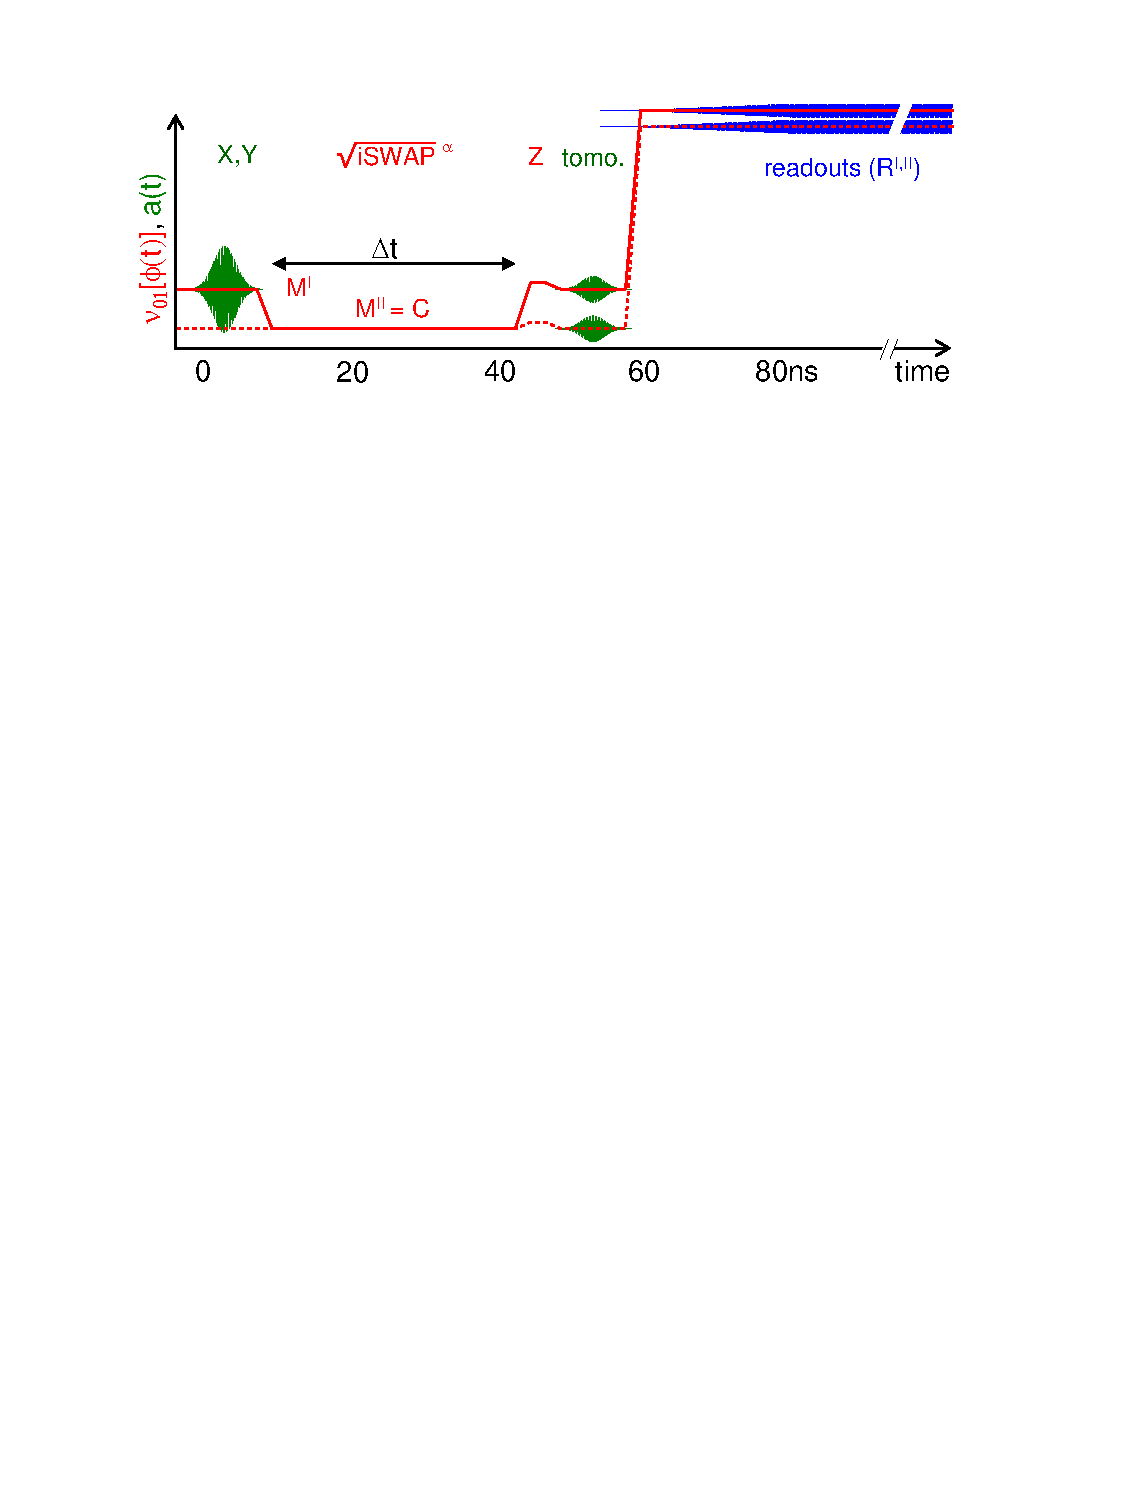
\includegraphics[width=0.8\textwidth]{./material/papers/iswap/figures/iswap_gate_pulse_sequence}
	\label{fig:ISwapPulseSequence}
	\caption{}
\end{figure}

\subsubsection{Violation of Bell's inequality}

\begin{figure}
	\centering
		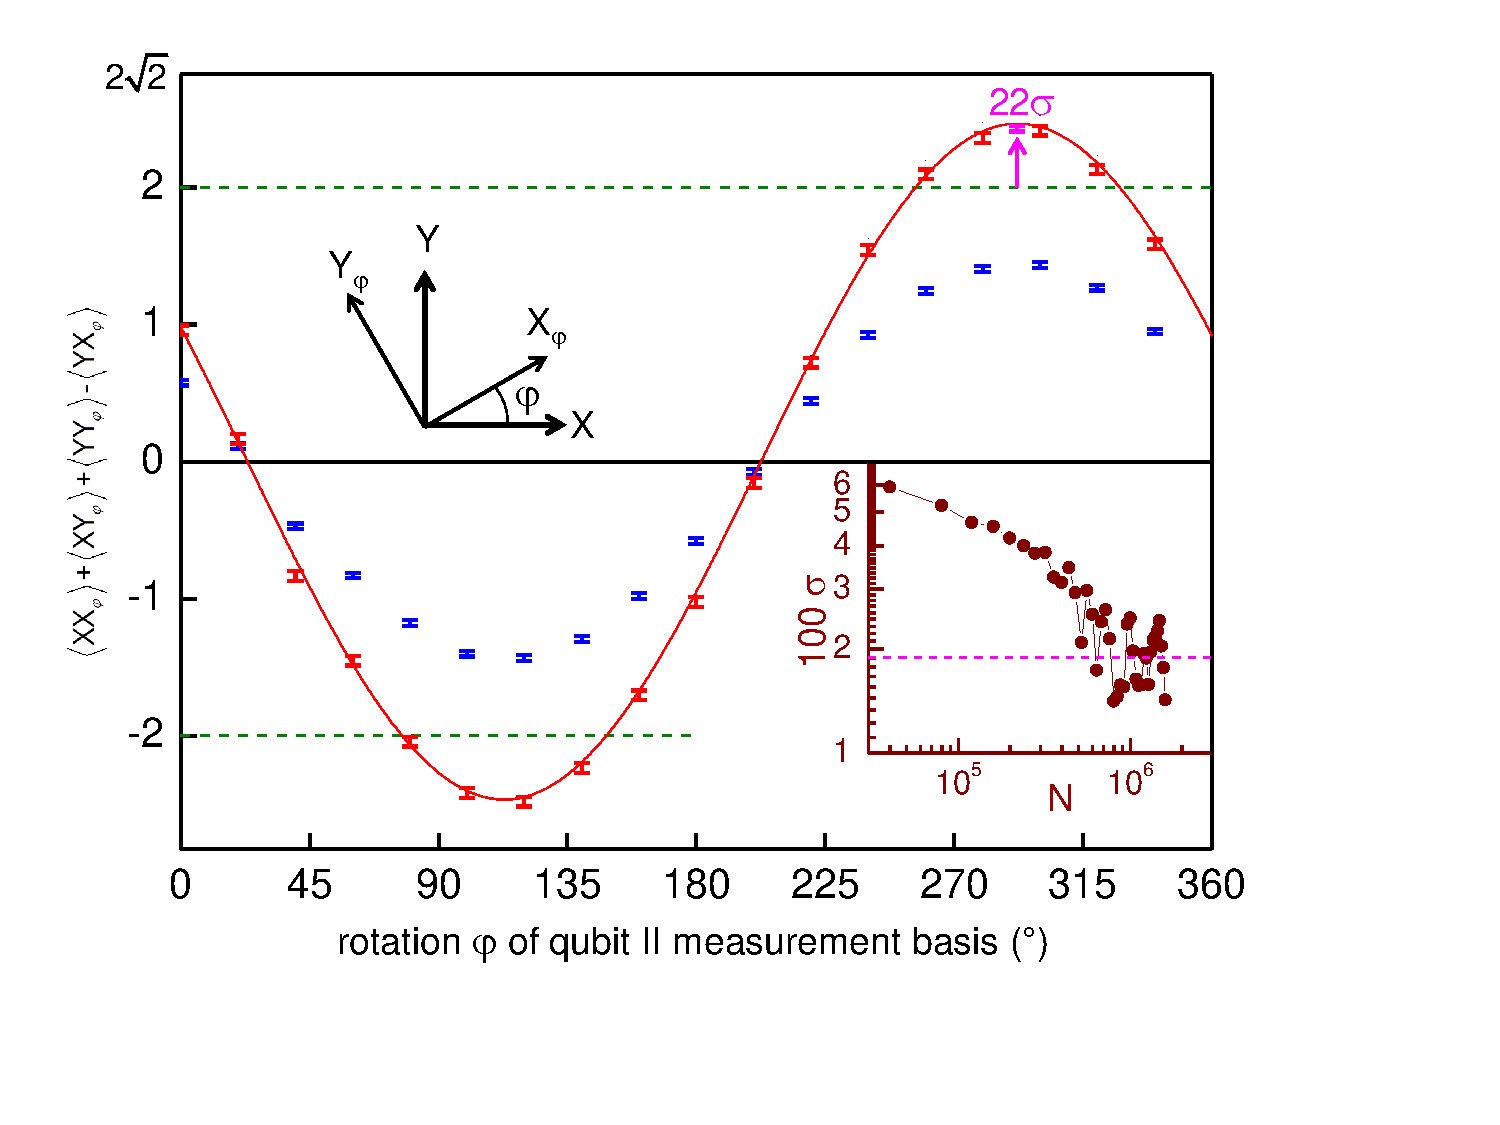
\includegraphics[width=0.8\textwidth]{./material/papers/iswap/figures/chsh}
	\label{fig:CHSH}
	\caption{}
\end{figure}

\subsection{Characterizing Quantum Processes}

\subsubsection{Introduction \& Principle}

\subsubsection{Implementation}

A quantum process can be described as a map $\mathcal{E} : \rho_\mathcal{H} \to \rho_\mathcal{H}$ that maps a density matrix $\rho$ defined in a Hilbert space $Q_1$ to another density matrix $\mathcal{E}(\rho)$ defined in a target Hilbert space $Q_2$ and fulfilling three axiomatic properties \cite{michael_a._nielsen_quantum_2000,haroche_exploring_2006}:

\begin{axiom}
$\mathrm{tr}\left[\mathcal{E}(\rho)\right]$ is the probability that the process represented by $\mathcal{E}$ occurs, when $\rho$ is the initial state.
\end{axiom}

\begin{axiom}
$\mathcal{E}$ is a {\it convex-linear map} on the set of density matrices, that is, for probabilities $\left\{p_i\right\}$,

  \begin{equation}
	  \mathcal{E}\left(\sum\limits_i p_i \rho_i\right) = \sum\limits_i p_i \mathcal{E}(\rho_i)
	\end{equation}
\end{axiom}

\begin{axiom}
$\mathcal{E}$ is a {\it completely-positive} map. That is, if $\mathcal{E}$  maps density operators of system $Q_1$ to density operators of system $Q_2$, then $\mathcal{E}(A)$ must be positive for any positive operator $A$. Furthermore, if we introduce an extra system $R$ of arbitrary dimensionality, it must be true that $(\mathcal{I}\otimes \mathcal{E})(A)$ is positive for any positive operator $A$ on the combined system $RQ_1$, where $\mathcal{I}$ denotes the identity map on system $R$.
\end{axiom}
As shown in \cite{michael_a._nielsen_quantum_2000}, any quantum process fulfilling these criteria can be written in the form

\begin{equation}
  \mathcal{E}(\rho) = \sum\limits_i E_i \rho E_i^\dagger \label{eq:process_operator_sum_representation}
\end{equation}
for some set of operators $\{ E_i \}$ which map the input Hilbert space to the output Hilbert space, and $\sum_i E_i^\dagger E_i \le I$.

Now, if we express the operators $E_i$ in a different operator basis $\tilde{E}_j$ such that $E_i = \sum_j a_{ij} \tilde{E}_{j}$ and insert into eq. (\ref{eq:process_operator_sum_representation}), we obtain

\begin{eqnarray}
 \mathcal{E}(\rho) & = & \sum\limits_i \sum\limits_j a_{ij} \tilde{E}_j \;\rho\; \sum\limits_k a_{ik}^* \tilde{E}_k^\dagger \\
& = & \sum\limits_{j,k}\tilde{E}_j \; \rho \; \tilde{E}_k^\dagger \sum\limits_i a_{ij} a_{ik}^* \\
& = & \sum\limits_{j,k}\tilde{E}_j \; \rho \; \tilde{E}_k^\dagger \; \chi_{jk} \label{eq:process_chi_representation}
\end{eqnarray}
where we defined $\chi_{jk} = \sum\limits_i a_{ij} a_{ik}^*$. This is the so-called $\chi$-matrix representation of the quantum process. Here, all the information on the process is contained in the $\chi$ matrix, which controls the action of the process-independent operators $\tilde{E}_i$ on the initial density matrix $\rho$.

Now, the goal of {\it quantum process tomography} is to obtain the coefficients of the $\chi$-matrix -- or any other complete representation of the process -- from a set of experimentally measured density matrices $\rho$ and $\mathcal{E}(\rho)$.

To achieve this, several techniques have been developed. The technique used in this work is the so-called {\it standard quantum process tomography (SQPT)}. This technique proceeds as follows:

\begin{enumerate}
\item Choose a set of operators $E_i$ that forms a full basis of $\mathcal{M}: Q_1 \to Q_2$. For n-qubit process tomography we usually choose $E_{i_1,i_2 \hdots i_n} = \sigma_{i_1}\otimes \sigma_{i_2}\hdots\otimes\sigma_{i_n}$, where $\sigma_i$ are the single-qubit Pauli operators and $i\in\{I,X,Y,Z\}$. 
\item Choose a set of pure quantum states $\ket{\phi_i}$ such that $\ket{\phi_i}\bra{\phi_i}$ span the whole space of input density matrices $\rho$. Usually, for a n-qubit system we choose $\phi = \{\ket{0},\ket{1},(\ket{0}+\ket{1})/\sqrt{2},(\ket{0}+i\ket{1})/\sqrt{2}\}^{\otimes n}$, where $^{\otimes n}$ denotes the n-dimensional Kronecker product of all possible permutations.
\item For each of the $\ket{\phi_i}$, determine $\mathcal{E}(\ket{\phi_i}\bra{\phi_i})$ by quantum state tomography. Usually we also determine $\ket{\phi_i}\bra{\phi_i}$ experimentally since the preparation of this state already entails small preparation errors that should be taken into account when performing quantum process tomography. 
\end{enumerate}

After having obtained the $\rho_i$ and $\mathcal{E}(\rho_i)$ one obtains the $\chi$-matrix by writing $\mathcal{E}(\rho_i) = \sum_j \lambda_{ij} \tilde{\rho}_j$, with some arbitrary basis $\tilde{\rho}_j$ and
letting $\tilde{E}_m \tilde{\rho}_j \tilde{E}_n^\dagger = \sum_k \beta_{jk}^{mn}\tilde{\rho}_k$. We can then insert into eq. (\ref{eq:process_chi_representation}) and obtain
\begin{eqnarray}
\sum\limits_k \lambda_{ik} \tilde{\rho}_k & = & \sum\limits_{m,n} \chi_{mn} \sum\limits_k \beta_{ik}^{mn} \tilde{\rho}_k  
\end{eqnarray}
This directly yields $\lambda_{ik} = \sum_{m,n}\beta_{ik}^{mn}\; \chi_{mn}$, which, by linear inversion,  gives $\chi$.

\subsubsection{The Kraus representation}

Besides the $\chi$-matrix representation, there is another useful way of expressing a quantum map, the so called {\it Kraus representation}, which is given as

\begin{equation}
 \mathcal{E}(\rho) = \sum\limits_i M_i \; \rho \; M_i^\dagger \label{eq:process_kraus_representation}
\end{equation}

It can be shown \citep{haroche_exploring_2006} that this sum contains at most $N$ elements, where $N$ is the dimension of the Hilbert space of the density matrix $\rho$. We can go from the $\chi$ representation to the Kraus representation by changing the basis $\tilde{E}_i$ such that

\begin{equation}
	\tilde{E}_i = \sum\limits_l a_{il}\; \breve{E}_l
\end{equation}

which, for eq. (\ref{eq:process_chi_representation}), yields

\begin{eqnarray}
 \mathcal{E}(\rho) & = & \sum\limits_{j,k} \sum\limits_l a_{jl} \breve{E}_l \; \rho \sum\limits_m a_{km}^* \breve{E}_m^\dagger \; \chi_{jk} \\
 & = & \sum\limits_{l,m}  \breve{E}_l \; \rho \; \breve{E}_m^\dagger \; \sum\limits_{j,k} a_{jl} a_{km}^* \chi_{jk} \label{eq:process_chi_transformed}
\end{eqnarray}

The last sum on the right side of eq. (\ref{eq:process_chi_transformed}) corresponds to a change of coordinates of the matrix $\chi$. Now, we can pick the $a$ such that $\chi$ is diagonal in the new basis $\breve{E}$ and obtain

\begin{eqnarray}
 \mathcal{E}(\rho) & = &  \sum\limits_{l} \lambda_l \breve{E}_l \; \rho \; \breve{E}_l^\dagger \\
& = &  \sum\limits_{l} M_l \; \rho \; M_l^\dagger
\end{eqnarray}
with $\lambda_l$ being the $l$-th eigenvalue of the $\chi$ matrix with the eigen-operator $\breve{E}_l$ and $M_{l} = \sqrt{\lambda_l} \breve{E}_l$.


\subsection{Realizing a Two-Qubit Gate}

\begin{figure}
   \centering
	 \includegraphics[width=1.\textwidth]{"./data/ct5/film of swap/pauli_set_vs_time_with_simulation"}
	 \caption[test]{testcaption}
	 \label{fig:swap_pauli_set_vs_time_with_simulation}
\end{figure}

\subsubsection{Principle}

\subsubsection{Implementation}

\subsubsection{Fidelity}

\subsubsection{Error Analysis}

%-Discuss the realization of a 2 qubit gate:
%  -Principle
%  -Implementation & Pulse Sequency
%  -Characterization through Quantum Process Tomography:
%     -Principles: State tomography, Pauli set, process tomography
%     -Discuss alternative representations of the process information:
%        -Chi matrix, Choi matrix, S, log S, Kraus operator representation
%  		-Errors: Discuss simulations, error models and possible reasons for discrepancies

\begin{figure}
	\centering
		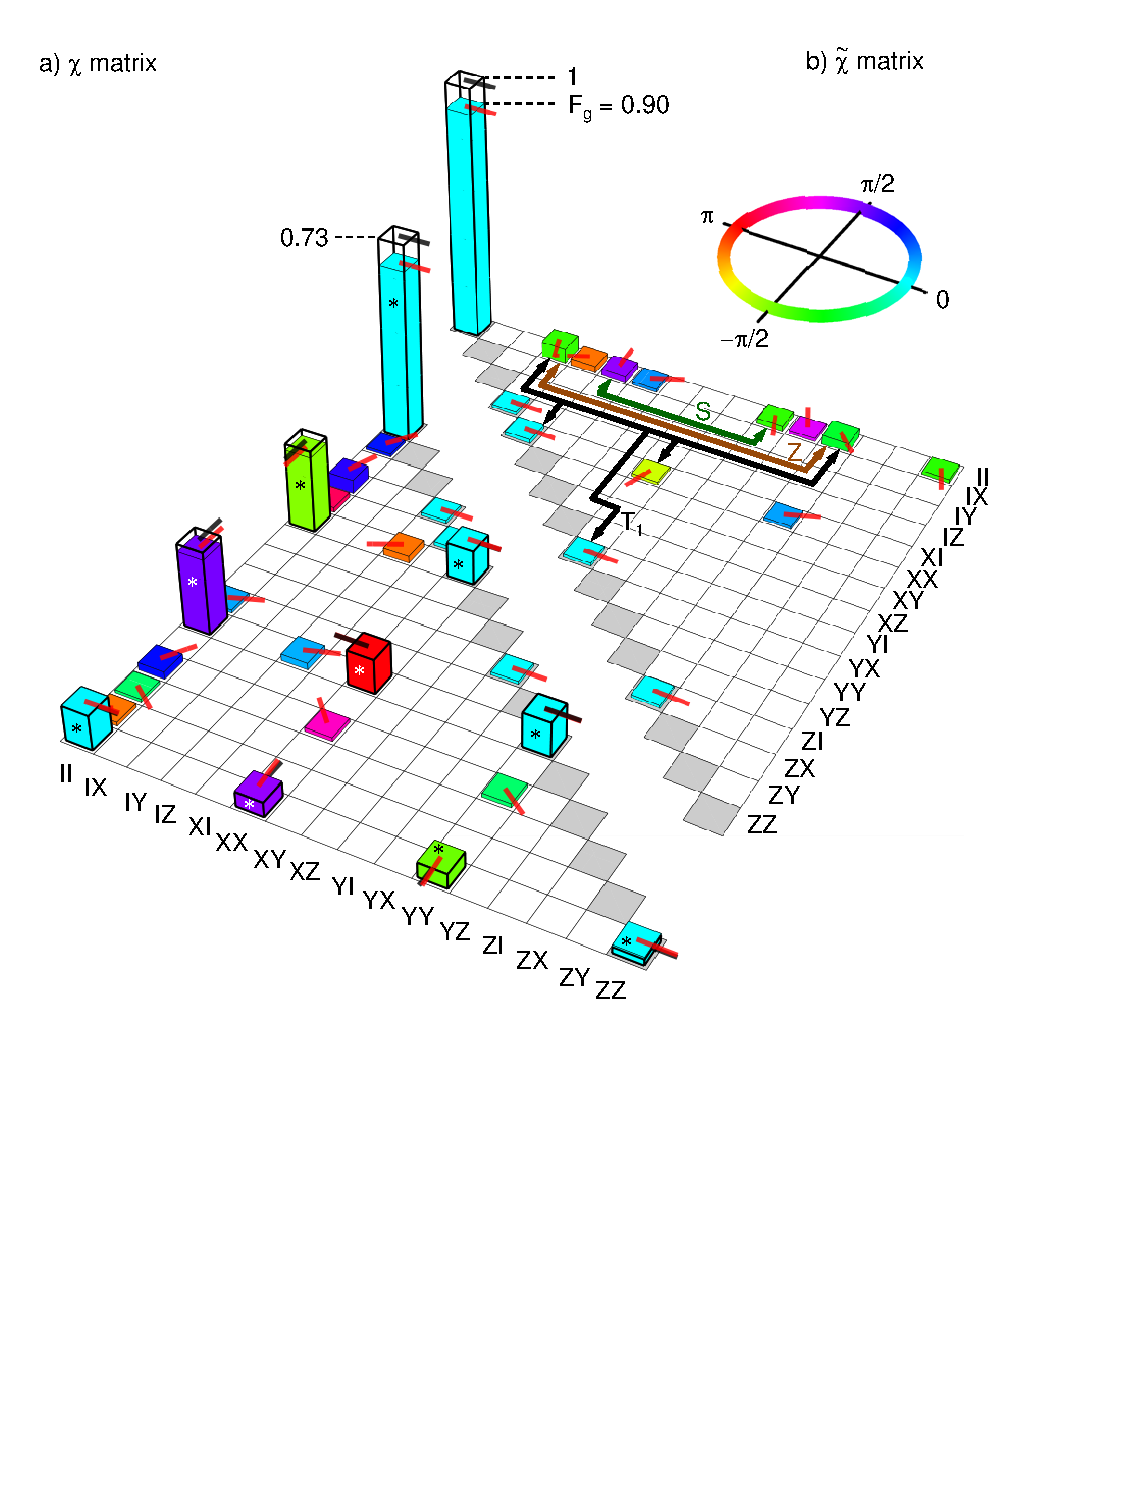
\includegraphics[width=1.\textwidth]{./material/papers/iswap/figures/chi_matrix_and_error_process}
	\label{fig:GateChiMatrixAndErrorProcess}
	\caption{}
\end{figure}


\section{Running Grover's Search Algorithm}

%Motivate this experiment:
% -Benchmark for superconducting quantum computers
% -Speed-up for searching in an unsorted database

\begin{figure}
	\centering
		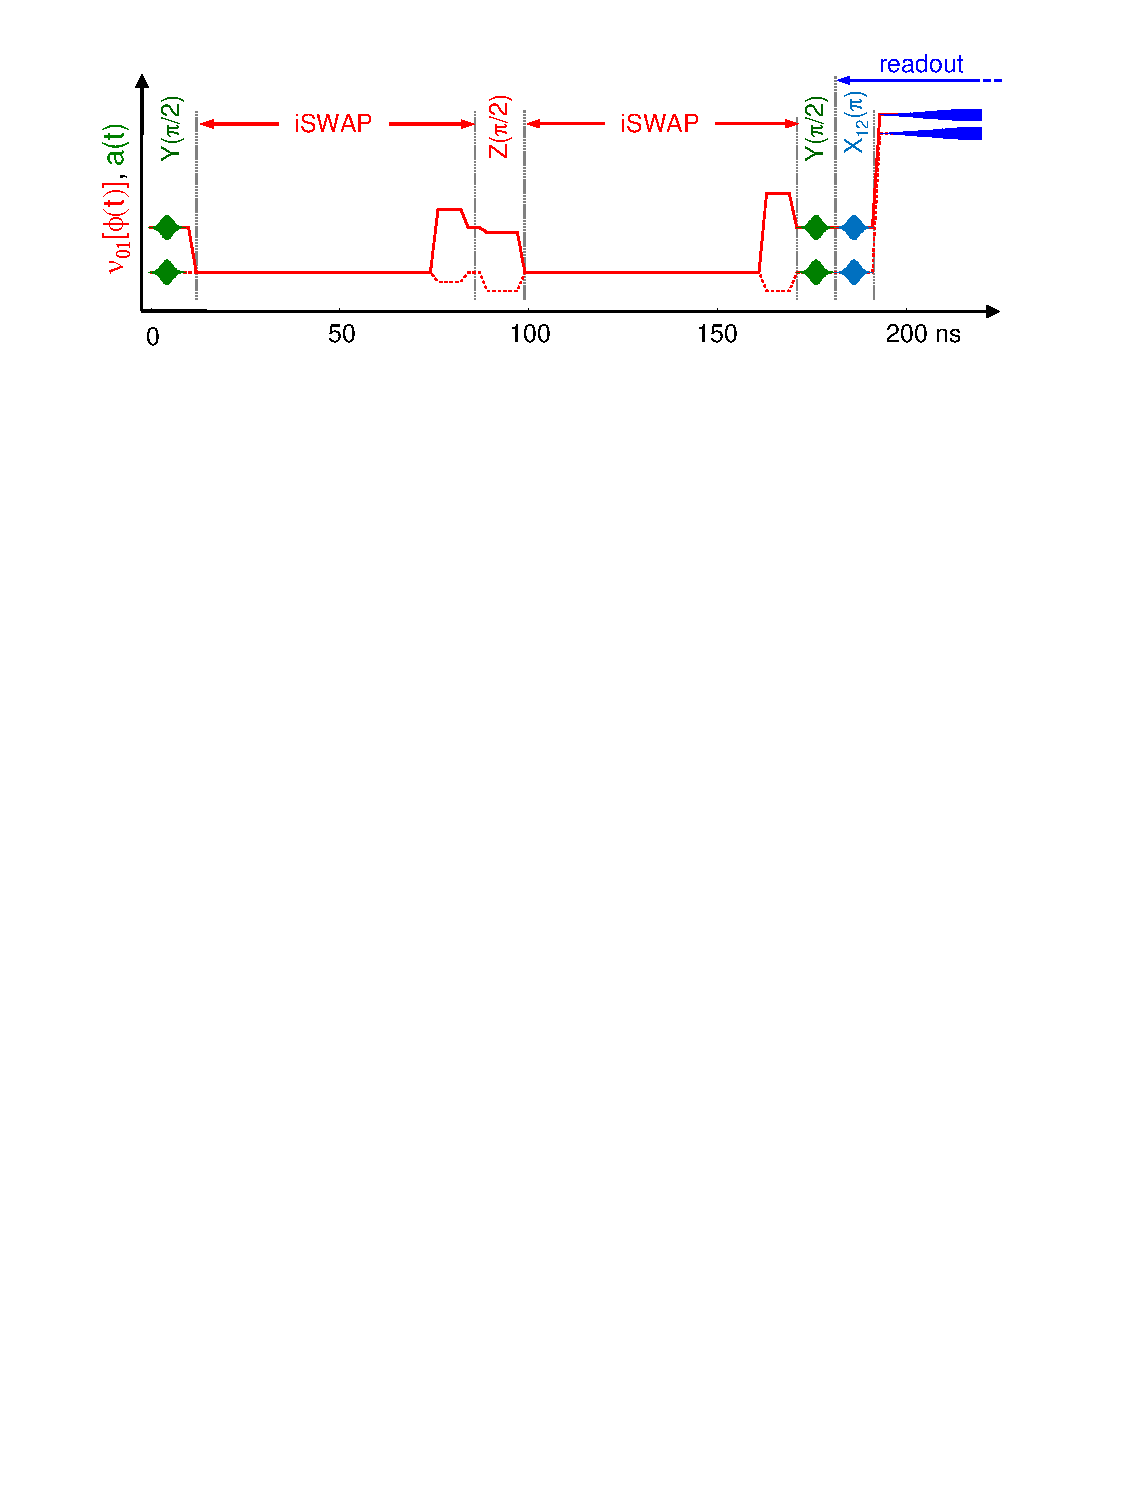
\includegraphics[width=1.\textwidth]{./material/papers/grover/figures/grover_algorithm_pulse_sequence}
	\label{fig:Grover3}
	\caption[Pulse sequence used for implementing Grovers search algorithm]{The pulse sequence used in realizing Grover's quantum search algorithm. First, a $Y_{\pi/2}$ pulse is applied to each qubit to produce the fully superposed state $1/2(\ket{00}+\ket{01}+\ket{10}+\ket{11})$. Then, an $i\mathrm{SWAP}$ gate is applied, followed by a $Z_{\pm \pi /2}$ gate on each qubit, which corrsponds to the application of the oracle function. The resulting state is then analyzed using another $i\mathrm{SWAP}$ gate and two $Y_{\pi/2}$ gates to extract the state which has been marked by the oracle function. Optionally, a $Y^{12}_{\pi}$ pulse is used on each qubit to increase the readout fidelity.}
\end{figure}

\subsection{Introduction \& Motivation}

\begin{enumerate}
  \item {\textbf Inputs:} An oracle function $\mathcal{O}$ which performs the operation $O\ket{x}\ket{q} = \ket{x}\ket{q\otimes f(x)}$, where $f(x) = \delta_{x,x_0}$
  \item {\textbf Outputs:} The marked state $x_0$
	\item Initialize the qubit register to the state: 
	$$\ket{\psi} \to \ket{0}^{\otimes n}\ket{0}$$
	\item Apply the Hadamard transformation to all of the qubits: 
	$$\ket{psi}\to \frac{1}{\sqrt{2^n}}\sum\limits_{x=0}^{2^n-1} \ket{x} \left[ \frac{\ket{0}-\ket{1}}{\sqrt{2}} \right]$$
	\item Apply the Grover iteration $R \approx [\pi \sqrt{2^n}/4]$ times:
	$$ \ket{\psi} \to \left[(2 \ket{\psi}\bra{\psi}-I)\mathcal{O}\right]^R \frac{1}{\sqrt{2^n}} \sum\limits_{x=0}^{2^n-1}\ket{x} \left[ \frac{\ket{0}-\ket{1}}{\sqrt{2}} \right] \approx \ket{x_0}\left[\frac{\ket{0}-\ket{1}}{\sqrt{2}}\right] $$
	\item Measure the first n qubits to obtain $x_0$
\end{enumerate}

For the Two-qubit case, this algorithm can be drastically simplified -- or ``compiled'' -- such that it runs without the ancilla qubit and in one single step of the Grover iteration:

\begin{enumerate}
  \item {\textbf Inputs:} An oracle function $\mathcal{O}$ which performs the operation $O\ket{x} =(-1)^{\delta_{x,x_0}}\ket{x}$, where $x_0$ is the marked state that is searched.
  \item {\textbf Outputs:} The marked state $x_0$
	\item 
\end{enumerate}

%-Explain the Grover experiment...
%		-Theoretical interest
%		-First demonstration in NMR
%   -Potential speed-up
%   -Details of the algorithm:
%     -Elementary operations
%     -Pulse shapes, corrections, ...

\begin{figure}
	\centering
		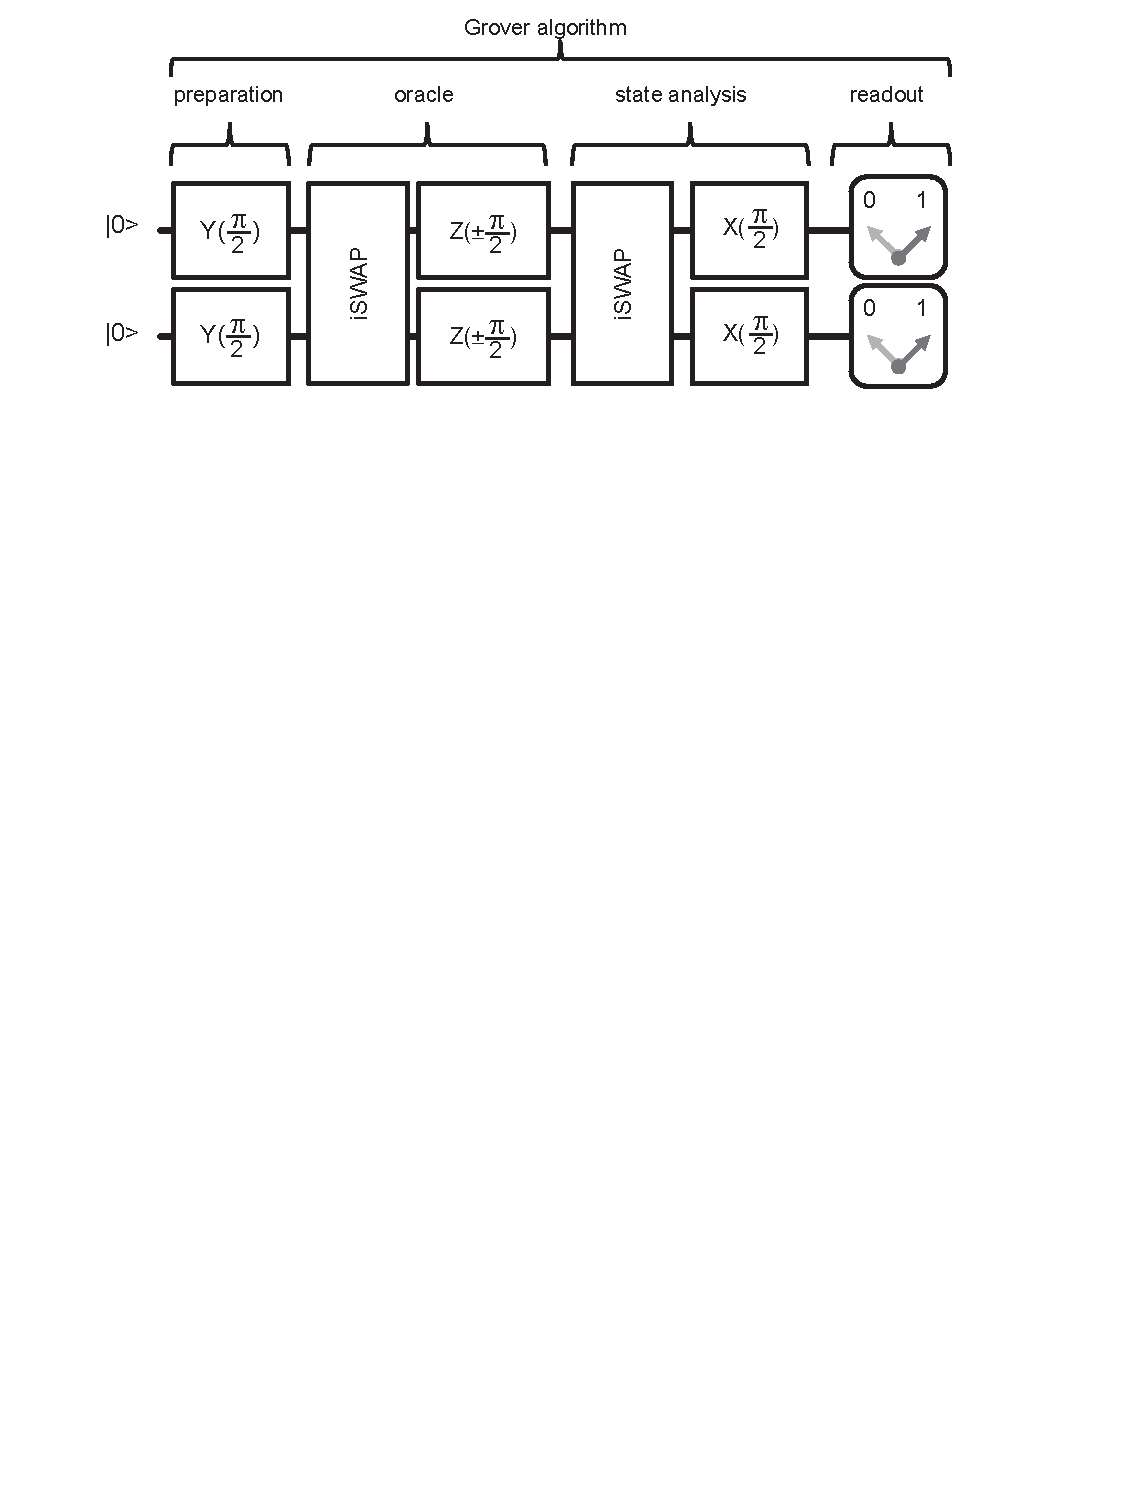
\includegraphics[width=1.\textwidth]{./material/papers/grover/figures/grover_algorithm_schematic}
	\label{fig:GroverAlgorithmSchematic}
	\caption{}
\end{figure}

\subsection{Experimental Implementation}

%-Show the implementation principle of the experiment.
%  -Break down the algorithm using the universal quantum gates that we've implemented

\subsection{Results}

%To Do:
%  -Create figures for all steps of the algorithm using Matplotlib
%  -Re-Analyze the data using Denis' Mathematica
%-Discuss the results and errors.

\begin{figure}
	\centering
		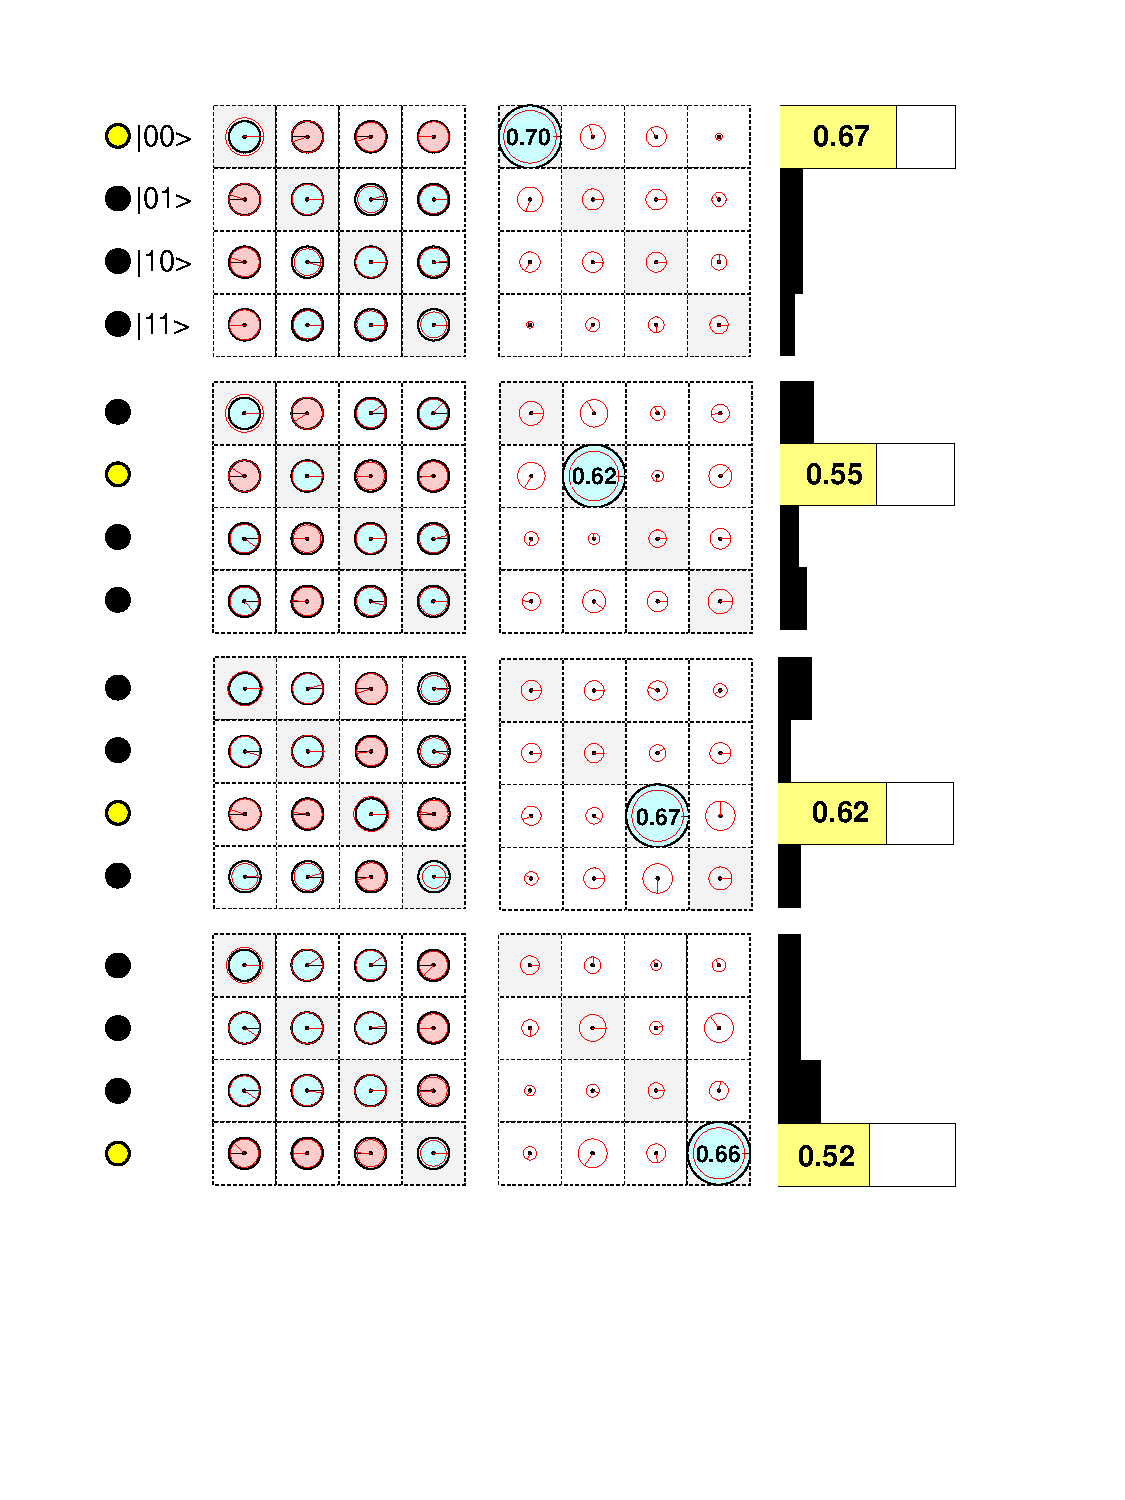
\includegraphics[width=1.\textwidth]{./material/papers/grover/figures/grover_algorithm_experimental_results}
	\label{fig:GroverAlgorithmExperimentalResults}
	\caption{}
\end{figure}

\subsubsection{Algorithm Fidelity}


\subsubsection{Single-Run Probabilities}

\subsubsection{Error Analysis}

\subsection{Conclusions}

%-Conclusions regarding quantum speed-up and applicability of results to larger-scale quantum computing.


\input{"scalable architecture"}

\chapter{Conclusions \& Outlook}

\section{Significance of Performed Experiments}

\section{Future Directions in Superconducting QC}

\subsection{3D Circuit Quantum Electrodynamics}

\subsection{Hybrid Quantum Systems}

\subsection{Quantum Error Correction}

\subsection{Quantum Feedback}


\appendix

\input{"appendix - modeling"}

\input{"appendix - data acquisition"}

\input{"appendix - fabrication"}

\bibliographystyle{apalike}

\stepcounter{chapter}

\addcontentsline{toc}{chapter}{\numberline {\thechapter} Bibliography}

\bibliography{thesis}

\end{document}
